\pdfminorversion=7
\documentclass[a4paper,fleqn]{cas-sc}
\usepackage{cmap}
\usepackage[T1]{fontenc}
\usepackage[utf8]{inputenc}

\usepackage{booktabs}
\usepackage{graphicx}
\usepackage{tabularx}
\usepackage[authoryear,longnamesfirst]{natbib}
\usepackage{afterpage}
\usepackage{placeins}
\usepackage{float}

\begin{document}
\def\floatpagepagefraction{1}
\def\textpagefraction{.001}
\let\WriteBookmarks\relax
\renewcommand\floatpagefraction{.85}
\renewcommand\topfraction{.85}
\renewcommand\bottomfraction{.9}
\renewcommand\textfraction{.1}
\setcounter{totalnumber}{4}
\setcounter{topnumber}{3}
\setcounter{bottomnumber}{1}

\shorttitle{From Requirements to Self-Healing Code}
\shortauthors{Dim et al.}

\title[mode=title]{From Requirements to Self-Healing Code: Grounded Extraction, Generation, and Compliance Enforcement for MVC-Based Python Applications}
\author[1]{{\.{I}}layda Dim}[orcid=0009-0006-4829-5452]
\ead{ilayda.dim@tedu.edu.tr}

\author[1]{Yaren Saklavc\i}[orcid=0009-0006-7148-5799]
\ead{yaren.saklavci@tedu.edu.tr}

\author[1]{Kaan Aytekin}[orcid=0009-0004-3176-6591]
\ead{kaan.aytekin@tedu.edu.tr}

\author[1]{Murat Karakaya}[orcid=0000-0002-9542-6965]
\cormark[1] 
\ead{murat.karakaya@tedu.edu.tr}

% --- ADRES (cas-sc için zorunlu güncel format) ---
\affiliation[1]{organization={Software Engineering Department, TED University},
    city={Ankara},
    country={Turkey}}

\cortext[cor1]{Corresponding author}

% --- ABSTRACT ---
\begin{abstract}
The practice of ``vibe coding,'' increasingly common in software development processes supported by Large Language Models (LLMs), can produce artifacts that violate intended architectural boundaries. This paper presents the \textit{MVC Test Orchestrator}, a prototype multi-agent pipeline that uses Software Requirements Specifications (SRS) as a single source of truth to derive Model-View-Controller (MVC)-oriented architectural artifacts via Retrieval-Augmented Generation (RAG), generate Python scaffolds, audit selected conformance rules using Abstract Syntax Trees (ASTs), and propose bounded repairs. The pipeline incorporates a Human-in-the-Loop (HITL) protocol to preserve developer oversight at key decision points. A descriptive evaluation was conducted on 20 purposively selected academic SRS documents using one Gemini 2.5 Flash configuration. The requirements artifacts achieved a macro-average BERTScore of 0.808 (SD\,=\,0.031), indicating semantic similarity between source SRS text and generated artifacts, but not requirement completeness. The analyzer achieved 98.8\% recall and 96.2\% precision on the fault-injection benchmark (F1\,=\,97.5\%). Among detected alerts for which repair was attempted, 92.6\% satisfied the recorded repair oracle. The rule-based scaffold transformation produced no recorded artifact discrepancies across all evaluated inputs (Scaffolder Error Rate, SER\,=\,0\%), and the macro-average Overall Consistency Score across three extraction runs was 70.6\% (SD\,=\,10.5). These findings support the feasibility of the tested pipeline for selected MVC conformance tasks within newly generated Python artifacts, but do not establish superiority, longitudinal prevention of architecture erosion, functional correctness, or generalization beyond the studied model, corpus, and Python rule set.
\end{abstract}

% --- KEYWORDS ---
\begin{keywords}
Architecture Erosion \sep Vibe Coding \sep Multi-Agent Systems \sep Retrieval-Augmented Generation \sep Abstract Syntax Tree \sep Self-Healing Systems
\end{keywords}

\maketitle

% ========================================================
% MAKALE GÖVDESİ
% ========================================================

\section{Introduction}
\label{sec:introduction}

Software engineering is a naturally complicated discipline, traditionally
ruled by a sequential, interconnected series of practices that include
requirements analysis, design, implementation, and testing. The Model-View-Controller (MVC) architecture, first introduced 
by Reenskaug~\citep{Reenskaug1979} and later formalized as a 
design pattern~\citep{Gamma1994}, remains one of the most 
widely adopted structural paradigms in software development.
By enforcing a clear separation of concerns across data management, user
interface, and control logic, MVC provides a principled foundation for
building maintainable, testable, and scalable systems. Even in the era
of AI-assisted development, this separation remains relevant; as code
generation accelerates, preserving architectural discipline becomes
increasingly critical.

However, the rapid integration of Large Language Models (LLMs) into the
development toolchain has been reported to erode this
discipline~\citep{Slater2025, Waseem2025, Ehsani2026}. AI-powered coding assistants
such as Cursor~\citep{Cursor2025}, GitHub Copilot~\citep{GitHubCopilot2025}, 
and OpenAI Codex~\citep{OpenAICodex2025} have significantly
accelerated implementation tasks~\citep{Hou2024}. However, this
speed may come at the expense of macro-level architectural
integrity, the structural coherence that governs inter-layer boundaries
and system-wide design consistency~\citep{Whiting2020}. The speed at which LLMs translate
complex business logic into functional code, while effective in isolated
benchmarks, deserves careful evaluation when applied to real-world,
architecture-sensitive projects.

This pattern is increasingly described as ``vibe
coding''~\citep{Fawzy2025}, an approach where developers rely heavily
on LLM outputs, generating code based on momentary decisions
rather than adhering to a defined architecture. The underlying danger is
that the generated code may function correctly in isolation, a function
may yield the correct output, a class may behave as expected, yet when
these components are integrated, the resulting structure often
contradicts the project's architectural principles and silently violates
inter-layer boundaries. LLM-generated code has been found to contain
structural and quality problems, such as poor exception handling,
undefined variables, and weak adherence to design rules, that can lead
to architectural drift in layered systems when combined without careful
review~\citep{Siddiq2024, Fawzy2025, Slater2025}. When developers
commit such violations to the codebase without adequate review,
technical debt accumulates without control.

Over time, this accumulation shows itself as Architecture
Erosion~\citep{Li2022}, defined as the progressive accumulation of
deviations between the intended architecture and the implemented
codebase. Architecture erosion goes beyond structural degradation: it restricts system
scalability and complicates the integration of new
requirements~\citep{Li2022}. Although various enforcement and
remediation approaches have been proposed to detect and address
architecture erosion~\citep{Li2022}, it remains a major unresolved
challenge in software engineering. As this accumulation stems from
architecturally non-compliant code introduced during development~\citep{Li2022},
we reason that mitigating it in AI-assisted workflows requires enforcement
mechanisms acting at the point of code generation, before such violations
can accumulate into long-term drift. Addressing this upstream,
point-of-generation problem, rather than measuring erosion's longitudinal
accumulation, is therefore the specific focus of the present study.

Existing tools have failed to mitigate this problem fully. Traditional
static analysis tools, such as SonarQube~\citep{SonarQube} and
Checkstyle~\citep{Checkstyle}, excel at detecting low-level syntactic
and stylistic anomalies; however, they largely overlook high-level
architectural deviations~\citep{Fontana2017}, such as inter-layer
responsibility leaks or MVC isolation violations. Furthermore, most current
architectural compliance tools require substantial manual preprocessing
to map the system to its intended architecture. This well-documented
barrier often leads practitioners to rely on informal, error-prone
inspection methods~\citep{Ali2018}. Another critical gap is the absence
of a structured, end-to-end traceability chain between Software
Requirements Specifications (SRS) and the generated code. While
existing traceability methods predominantly rely on Information
Retrieval (IR) techniques, they continue to exhibit significant
limitations in terms of full automation and seamless integration into
modern development workflows~\citep{Koboyatshwene2025}.

We propose the \textit{MVC Test Orchestrator} to address this gap, a
multi-agent system designed to preserve and enforce MVC architectural
integrity across the AI-assisted development workflow and built on an
``Architecture-First'' philosophy, wherein all design and code
generation decisions are anchored to and constrained by the SRS before
any implementation step begins. Concretely, the framework: (i)~extracts
MVC components from unstructured SRS text via RAG-grounded multi-agent
orchestration (\texttt{/extract}); (ii)~generates rule-based project
scaffolds that enforce MVC layer boundaries at the file-system level
(\texttt{/scaffold}); (iii)~detects inter-layer architectural violations
through AST-based static analysis (\texttt{/audit}); and
(iv)~autonomously remediates identified violations within the boundaries
of the established Architectural Map (\texttt{/fix}). The system
establishes the SRS document as the single source of truth, governing
this entire workflow from requirements analysis through autonomous
remediation. Rather than functioning as a fully autonomous black box,
the system employs a Human-in-the-Loop (HITL) architecture that
preserves developer oversight and strategic authority at every stage,
acknowledging that LLM-based agents can approximate but not fully
guarantee rule-bound behavior. Underlying these mechanisms is what we
term a Safety-Layered Architecture: rule-based components (scaffolding,
AST-based auditing) are interleaved with the LLM's generative steps,
aiming to bound their stochastic variability within verifiable
architectural constraints.

\smallskip\noindent\textbf{Scope.} The prototype is intended to support MVC structural conformance in newly generated Python artifacts. The study does not observe the longitudinal evolution of a production codebase and therefore does not directly measure architecture erosion, architectural drift over time, or technical-debt accumulation.

This paper makes three contributions. First, we present a multi-agent
architecture that automates the complete MVC lifecycle, from SRS
ingestion to self-healing remediation. This architecture combines
RAG-based semantic grounding with rule-based scaffolding and AST-driven
auditing under a HITL oversight protocol. Second, we introduce an
eight-metric evaluation framework spanning both LLM-based generative
stages and rule-based pipeline stages. These metrics include Semantic
Consistency (BERTScore), Architectural Component Extraction Score
(ACES), Scaffolder Error Rate (SER), Violation Detection Recall and
Alert Confirmation Precision (VDR/ACP), Repair Success among Detected
Alerts and end-to-end Repair Success Rate (RSDA/RSR\textsubscript{e2e}), and
Consistency Score (CS). Third, we report empirical results across 20
SRS documents of varying domain and complexity. The system achieves an
extraction score of 74.0\%, a violation detection recall of 98.8\%
(96.2\% precision), a remediation success rate of 92.6\% among detected
violations, a 0\% scaffolding error rate across all evaluated
documents, and a 70.6\% consistency score across three independent
iterations per document.

The remainder of this paper is organized as follows: Section~\ref{sec:related_work} reviews
the relevant literature, Section~\ref{sec:methodology} describes the proposed methodology
and system architecture, Section~\ref{sec:experiment} presents the experimental
design---including the five Research Questions (RQ1--RQ5) that
structure the evaluation---and the evaluation metrics, Section~\ref{sec:results}
reports the experimental results, Section~\ref{sec:discussion} discusses the findings,
Section~\ref{sec:limitations} addresses the limitations and threats to validity, Section~\ref{sec:conclusion}
concludes the study, and Section~\ref{sec:future} outlines potential directions for
future research.

\smallskip\noindent\textbf{Extension beyond the preliminary conference paper.} This journal article substantially extends the five-case preliminary study reported by \cite{dim2026mvc}. The evaluation corpus is expanded from 5 to 20 SRS documents, and the architecture is redesigned around three specialized Architect Agents instead of one. This study also adds an autonomous remediation stage that was not present in the conference version, and replaces the earlier AI-as-a-Judge evaluation with a five-expert human panel supported by an Inter-Rater Reliability analysis. The evaluation framework itself grows from five simple metrics to eight, organized around five research questions (RQ1--RQ5) not present in the earlier work. The conference paper is cited wherever the original extraction and scaffolding concepts are described; reused material is limited to the underlying problem framing, the core RAG mechanism, and the public code repository.
\section{Related Work}
\label{sec:related_work}

This section reviews five interconnected areas that motivate the
design of the MVC Test Orchestrator. It first examines traditional
approaches to architectural enforcement and static analysis,
highlighting their structural limitations. It then surveys the
evolution of LLM-based code generation and its implications for
architectural integrity. Next, it reviews requirement-to-architecture
traceability frameworks and their limitations in supporting automated,
end-to-end compliance. It also assesses automated program repair and
code remediation, and finally discusses Human-AI collaboration in
software engineering. Together, these strands reveal the specific gap
the proposed system is designed to address.

% -----------------------------------------------------------------
\subsection{Traditional Architectural Enforcement and Static Analysis}
\label{sec:related_static}
% -----------------------------------------------------------------

Software architecture serves as a foundational building block for
satisfying a system's quality attributes and enforcing its structural
constraints. As software systems and their component modules evolve,
the separation between the intended architectural design and the
implemented codebase becomes an ongoing challenge. Defined in the
literature as Architecture Erosion \citep{Li2022}, this
deviation risks the integrity of the system's modular structure.
Beyond structural degradation, it increases system vulnerabilities
and limits extensibility, complicating the integration of new
requirements \citep{Li2022}. Although various monitoring and
remediation strategies have been proposed to mitigate this decay
\citep{deSilva2012}, the interplay of technical and non-technical
factors keeps architecture erosion among the major unsolved problems in software
engineering \citep{Li2022}.

Historically, approaches to preserving architectural integrity have
relied on modularization, information hiding \citep{Parnas1972}, and
optimized coupling and cohesion \citep{Yourdon1979}.
Scenario-based evaluation frameworks, including SAAM \citep{Kazman1994}
and ATAM \citep{Kazman2000}, were developed to identify architectural
risks before implementation and to verify alignment between quality
requirements and the proposed design. However, most traditional methods
fail to establish a consistent link between quality attributes and
architectural artifacts, and often depend on manual or informal
processes \citep{Dobrica2002}. In practice, failure to strictly capture
high-level architectural artifacts---documents that represent the
macro-level system design---often prevents these abstractions from
guiding the implementation and reuse of low-level components
\citep{Lung1997}.

Currently, automated tools used to ensure architectural compliance,
such as SonarQube \citep{SonarQube} and Checkstyle
\citep{Checkstyle}, focus almost exclusively on low-level code
anomalies, including syntactic irregularities and stylistic errors.
Consequently, high-level structural violations affecting the system's
organizational logic---such as invalid dependencies that violate
architectural rules---are detected only to a limited extent \citep{Fontana2017}.
Developers' reluctance to adopt formal architectural compliance tools
has been attributed in the literature to the substantial effort
required to map a system to its architecture \citep{Ali2018}. Existing commercial solutions typically
require substantial manual preprocessing to map the codebase to the
intended architecture---a configuration overhead that \citet{Ali2018} identify as a key adoption barrier, often resulting in
informal, error-prone verification methods.

Operating under a ``Just-In-Time'' paradigm, tools like JITTAC
\citep{Buckley2013} represent some of the most proactive traditional
solutions, as developers are informed about the architectural
implications of their modifications during coding. By employing
real-time Reflexion Modeling \citep{Murphy2001} techniques, they reduce
architectural drift by enforcing consistency between the designed
architecture and the executed code. Nevertheless, even with
sophisticated tools like JITTAC, the target architectural model must
still be manually defined by software architects, and source code
elements must be explicitly mapped to this abstraction
\citep{Buckley2013}.

Recent studies \citep{Fuchs2025, Helmi2025} show that LLM-based
approaches have significant potential to autonomously extract and
isolate architectural components from Software Requirement
Specifications (SRS), thereby addressing manual mapping bottlenecks.
To reduce the risk of architectural drift, however, bidirectional
traceability between documented requirements and code-level structural
constraints should be coupled with autonomous remediation.

Architecture conformance approaches differ from general code-quality analyzers such as SonarQube~\citep{SonarQube} and Checkstyle~\citep{Checkstyle}. Reflexion models~\citep{Murphy2001} and just-in-time conformance techniques~\citep{Buckley2013} compare implemented dependencies with an explicitly defined target architecture, while architecture-test and dependency-rule approaches encode admissible relations as executable constraints~\citep{Pruijt2017}. These families provide stronger architectural baselines than style-oriented analyzers, but typically require developers to specify or maintain the target model. The present prototype explores whether an SRS-derived MVC map can reduce that setup burden; it does not replace or empirically outperform established conformance tools in this study.

The tools and methods reviewed in this section share a common
limitation: they either operate at too low an abstraction level to
capture MVC-layer violations or require substantial manual
configuration, undermining automation. The MVC Test Orchestrator
addresses this gap by combining SRS-grounded requirement analysis with
automated architectural auditing, eliminating the need for manual
model definition while maintaining developer management through a
Human-in-the-Loop design. Unlike JITTAC and similar tools, which
require architects to manually define the target model before analysis
begins, the MVC Test Orchestrator derives the model automatically from
the SRS document. Detection is also scoped to MVC-specific inter-layer
violations rather than general code anomalies, removing the manual
configuration step identified as a key adoption barrier by \citet{Ali2018}.

% -----------------------------------------------------------------
\subsection{Large Language Models in Software Engineering}
\label{sec:related_llm}
% -----------------------------------------------------------------

The integration of Large Language Models (LLMs) into the software
development lifecycle has driven a major shift in automated code
generation and developer productivity. Despite the well-documented
risks to logical consistency and contextual accuracy \citep{Siddiq2024},
the speed of these models has supported their general adoption across
the industry \citep{Hou2024}. Nevertheless, \citet{Slater2025} reports that smaller, open-weight
LLMs exhibit a critical limitation in their ability to naturally
understand and enforce global architectural constraints that control
the macro-level system, whereas larger proprietary models demonstrate
markedly higher conformance.

Current research suggests that while LLMs excel at generating
syntactically correct and functionally feasible code snippets within a
localized context, they may systematically violate layered architectural
rules and isolation principles at the macro level
\citep{Slater2025, Zhu2026}. Particularly within ``vibe coding'' workflows, AI-generated
implementations that conflict with the project's architectural
blueprints are reported to accelerate the accumulation of
Architecture Erosion and technical debt
\citep{Slater2025, Waseem2025, Ehsani2026}. Developers' over-reliance on
AI-generated outputs often allows these structural violations to enter
the codebase without strict architectural inspection, fueling an
uncontrolled accumulation of technical debt \citep{Huang2026}.

Consequently, prompt-level engineering or simple fine-tuning alone may
be insufficient to preserve architectural integrity
\citep{Dente2026, Zhu2026}. This gap underscores the need for an
``architectural orchestrator'' mechanism, one capable of constraining
the generative output rate of LLMs by establishing a structured,
bidirectional bridge between Software Requirement Specifications (SRS)
and code-level structural constraints, while also including autonomous
remediation capabilities.

The MVC Test Orchestrator directly addresses this need by imposing
architectural constraints before code generation begins, grounding each
generation step in SRS-derived requirements rather than relying on the
model to infer architectural rules independently. This structural
approach to constraint enforcement, discussed further in Section~\ref{sec:experiment},
represents a departure from existing LLM coding assistants that lack a
formal architectural representation \citep{Cervantes2026}.

% -----------------------------------------------------------------
\subsection{Requirement-to-Architecture Traceability and RAG}
\label{sec:related_traceability}
% -----------------------------------------------------------------

Traceability, defined as the process of establishing and maintaining
bidirectional relationships between software requirements,
architectural artifacts, and source code, is a critical determinant of
product quality and effective change management \citep{Li2022}. A
recent systematic literature review spanning 2013 to 2024 indicates
that, while most traceability methods rely heavily on Information
Retrieval (IR) techniques, these approaches still exhibit severe
limitations in full automation and seamless integration with modern,
iterative development approaches such as Agile and DevOps
\citep{Koboyatshwene2025}. Furthermore, the scarcity of comprehensive,
end-to-end tool support and the tendency to evaluate these methods on
static, legacy datasets rather than dynamic industrial case studies
continue to slow industrial adoption and limit empirical reliability.

The built-in semantic gap between high-level architectural
documentation and low-level source code constitutes a fundamental
obstacle to establishing robust traceability links. Traditionally,
bridging this gap required the manual construction of software
architectural models---a highly labor-intensive, error-prone, and
costly effort \citep{Clements2002}. However, recent advances in Large
Language Models (LLMs) have enabled the automated extraction of
architectural entities and their relationships directly from both
natural-language documentation and source code. By avoiding the need
for manual modeling, this capability effectively bridges the semantic
gap and enables the generation of high-fidelity traceability links
\citep{Fuchs2025}.

These advances provide a solid foundation for the use of
Retrieval-Augmented Generation (RAG) architectures in software
engineering \citep{Hey2025}. In this context, RAG utilizes autonomously
extracted architectural components and formal requirement
specifications as a semantic ``grounding'' mechanism. This enables
thorough verification of code-level architectural integrity against the
system's dynamic documentation (SRS documents updated
iteratively). Ultimately, this integration harmonizes the generative
capabilities of LLMs with defined architectural constraints,
effectively transforming traceability from a passive, backward-looking
tracking mechanism into an active, real-time remediation process.

The MVC Test Orchestrator builds directly on these advances by
embedding RAG-based semantic retrieval as its primary grounding
mechanism. Rather than treating traceability as a passive
record-keeping activity, the proposed system uses SRS-derived
requirements as a live semantic anchor against which generated code is
continuously verified, closing the automation gap identified in current
IR-based approaches. In this way, automated forward traceability from requirements to code---a
gap that existing methods fail to close---is achieved through the combination
of LLM-based extraction and structured architectural auditing
\citep{dim2026mvc}.

% -----------------------------------------------------------------
\subsection{Automated Program Repair and Code Remediation}
\label{sec:related_apr}
% -----------------------------------------------------------------

While traditional debugging and maintenance methodologies mainly focus
on generating localized patches driven by specific test scenarios, the
advent of generative AI has advanced this area toward the
conceptualization of ``self-healing'' software systems. This
transition forms the core of modern Automated Program Repair (APR)
frameworks, such as RepairAgent \citep{Bouzenia2025} and ChatRepair
\citep{Xia2024}, which are engineered to minimize maintenance overhead
and substantially enhance system reliability. Recent empirical work by
\citet{Khlaisamniang2023} demonstrated that
autonomous remediation mechanisms can effectively address
component-level failures in large-scale systems by leveraging
generative AI for anomaly detection, code generation, and
automated debugging. Such approaches significantly reduce the
need for manual intervention while preserving core system
functionality and operational efficiency.

However, while the automated remediation of localized, syntax-level
defects has become increasingly viable, resolving macro-level
structural debt and architectural ``smells'' \citep{Fontana2017}
remains a highly complex challenge. A recent investigation by
\citet{Pandini2025} highlighted that LLMs exhibit considerable
capability in formulating refactoring strategies to mitigate complex
structural flaws, such as Cyclic Dependencies (CD). Their study
revealed that RAG-enhanced LLM outputs were preferred by 73\% of
participants in qualitative interviews, primarily because they offered
improved solution structure and clearer step-by-step reasoning in the
generated refactoring proposals.

To handle the contextual complexity present in architectural
remediation, the use of multi-agent architectures has been suggested to be
important for preserving system integrity
\citep{Oueslati2025, Xu2025, Batole2025}. The systematic division of
responsibilities---for instance, designating one agent to identify the
optimal dependency to separate, while another executes the
corresponding code refactoring---yields more reliable outcomes when
resolving complex dependency cycles \citep{Pandini2025}. These findings
suggest that coordinated LLM-driven remediation holds promise for
addressing not merely functional anomalies, but also deep structural
deviations that violate a project's foundational architectural
constraints; however, current benchmarks indicate this capability
remains inconsistent, with even the best-performing agents resolving
fewer than half of identified architectural smells and occasionally
introducing new violations \citep{Dinu2026}.

Existing APR frameworks, such as RepairAgent and ChatRepair, operate
without a fixed architectural reference, which means a local fix can
introduce a new structural violation elsewhere in the codebase. The
Fixer Agent in the MVC Test Orchestrator avoids this by restricting
all repairs to the violations flagged by the AST-based static
analyzer; it cannot modify the rule-based project scaffold or the Architectural Map
during patching. The practical effect of this constraint is measured
in Section~\ref{sec:results} through the RSDA and RSR\textsubscript{e2e} metrics.

% -----------------------------------------------------------------
\subsection{Human-AI Collaboration in Software Engineering}
\label{sec:related_hitl}
% -----------------------------------------------------------------

The deployment of AI agents within software engineering workflows is
increasingly shifting away from fully autonomous ``black-box''
approaches and toward Human-in-the-Loop (HITL) hybrid systems. \citet{Sera2025} emphasize that within dynamic,
self-managing architectures, human oversight during the ``Plan''
phase of the classical Monitor, Analyze, Plan, Execute,
Knowledge (MAPE-K) cycle \citep{Kephart2003} is essential for safeguarding
quality attributes and reducing unintended behavior. This
collaborative model positions AI agents as autonomous executors of
operational tasks while reserving strategic governance to human
developers, ensuring the system does not unintentionally deviate from
its intended architectural constraints.

This architectural imperative is supported by current Human-in-the-Loop
LLM-based frameworks. Existing literature demonstrates that permitting
AI agents to execute complex planning and coding tasks without human
validation significantly increases the risk of generating convincing
but erroneous outputs (hallucinations) \citep{Ji2023}.
Ultimately, the effectiveness of human-AI collaboration is dependent
on the transparency and explainability of the AI's recommendations.
Empirical analyses by \citet{Pandini2025} indicate that
developers adopt AI-generated architectural refactoring suggestions
with significantly greater confidence when the proposals are
accompanied by explicit, step-by-step reasoning, thereby directly
enhancing the perceived utility of the intervention.

Building on this collaborative context, the authors initially
introduced the foundational baseline of the MVC Test
Orchestrator~\citep{dim2026mvc}. The preliminary architecture presented at the
International Informatics and Software Engineering Conference (IISEC) constrained LLM outputs using structured, rule-based
scaffolding, establishing the SRS document as the definitive source of
truth. The present study extends this initial framework, as detailed in
Section~\ref{sec:introduction}. Through these advancements, human-AI
interaction is elevated from a passive validation checkpoint into a
proactive, autonomous, and architecturally grounded management process.

What distinguishes the current work from the HITL frameworks surveyed
here is the role of human oversight in the process. In most HITL
systems, humans review AI output after it is generated. In the MVC
Test Orchestrator, the SRS, a human-authored document, defines the
architectural boundaries before any generation begins, so developer
intent is built into the system from the start rather than checked
after the fact.

Taken together, the literature reviewed across
Sections~\ref{sec:related_static} through~\ref{sec:related_hitl}
reveals a consistent and critical gap in the current state of the art.
Traditional static analysis tools operate at too low an abstraction
level to detect MVC-layer violations, while scenario-based evaluation
frameworks remain heavily dependent on manual configuration. LLM-based
code generation, despite its productivity gains, has been shown to
systematically undermine macro-level architectural constraints in the
absence of structured oversight. Existing traceability methods lack
the automation and dynamic integration needed to support modern
development workflows, and current automated repair mechanisms address
localized defects without accounting for broader architectural
coherence. The MVC Test Orchestrator is proposed to address this
combination of limitations. By grounding code generation in
SRS-derived requirements through RAG-based semantic retrieval,
enforcing MVC architectural boundaries through AST-based static
analysis, and embedding human oversight at each decision point through
a HITL design, the proposed system offers an integrated response to
challenges that existing approaches address only in isolation. Rather
than optimizing a single dimension of the development pipeline, the
aim is to establish a traceable, auditable, and architecturally
coherent workflow from requirements to implementation.
\section{Proposed Methodology}
\label{sec:methodology}

This section details the technical infrastructure and operational pipeline of the proposed MVC Test Orchestrator. To mitigate the structural degradation and risks associated with ``vibe coding'' highlighted in the previous section, the system is fundamentally anchored in the classical Software Development Life Cycle (SDLC). The fundamental phases of (1) Requirements Analysis, (2) Architectural Design, (3) Implementation (Coding), and (4) Review, traditionally executed by human experts, are automated within this architecture through a specialized multi-agent orchestration. Crucially, this automation avoids an opaque ``black-box'' paradigm. Because each stage is designed to consistently produce transparent, human-readable artifacts (JavaScript Object Notation (JSON) and Markdown), developers retain the strategic authority to inspect, override, or manually resume the process at any point. The subsequent subsections explain how these traditional MVC paradigm steps are rendered autonomous.

\subsection{System Architecture and Multi-Agent Orchestration}

The high-level structural organization of this Architecture-First pipeline (Section~\ref{sec:introduction}) is illustrated in Figure~\ref{fig:31}. Rather than relying on a monolithic, zero-shot LLM prompt, the system is constructed upon a structured, requirements-driven foundation. Through this pipeline, the Software Requirements Specification (SRS) document is structurally positioned as the ultimate authority and the single source of truth throughout the entire development lifecycle. This foundational perspective is explicitly designed to detect MVC conformance violations in generated artifacts. Consequently, instead of producing disjointed classes and stochastic code snippets, the system synthesizes a traceable and verifiable structural hierarchy grounded directly in the specific constraints of the SRS document.

\begin{figure}[pos=h]
\centering
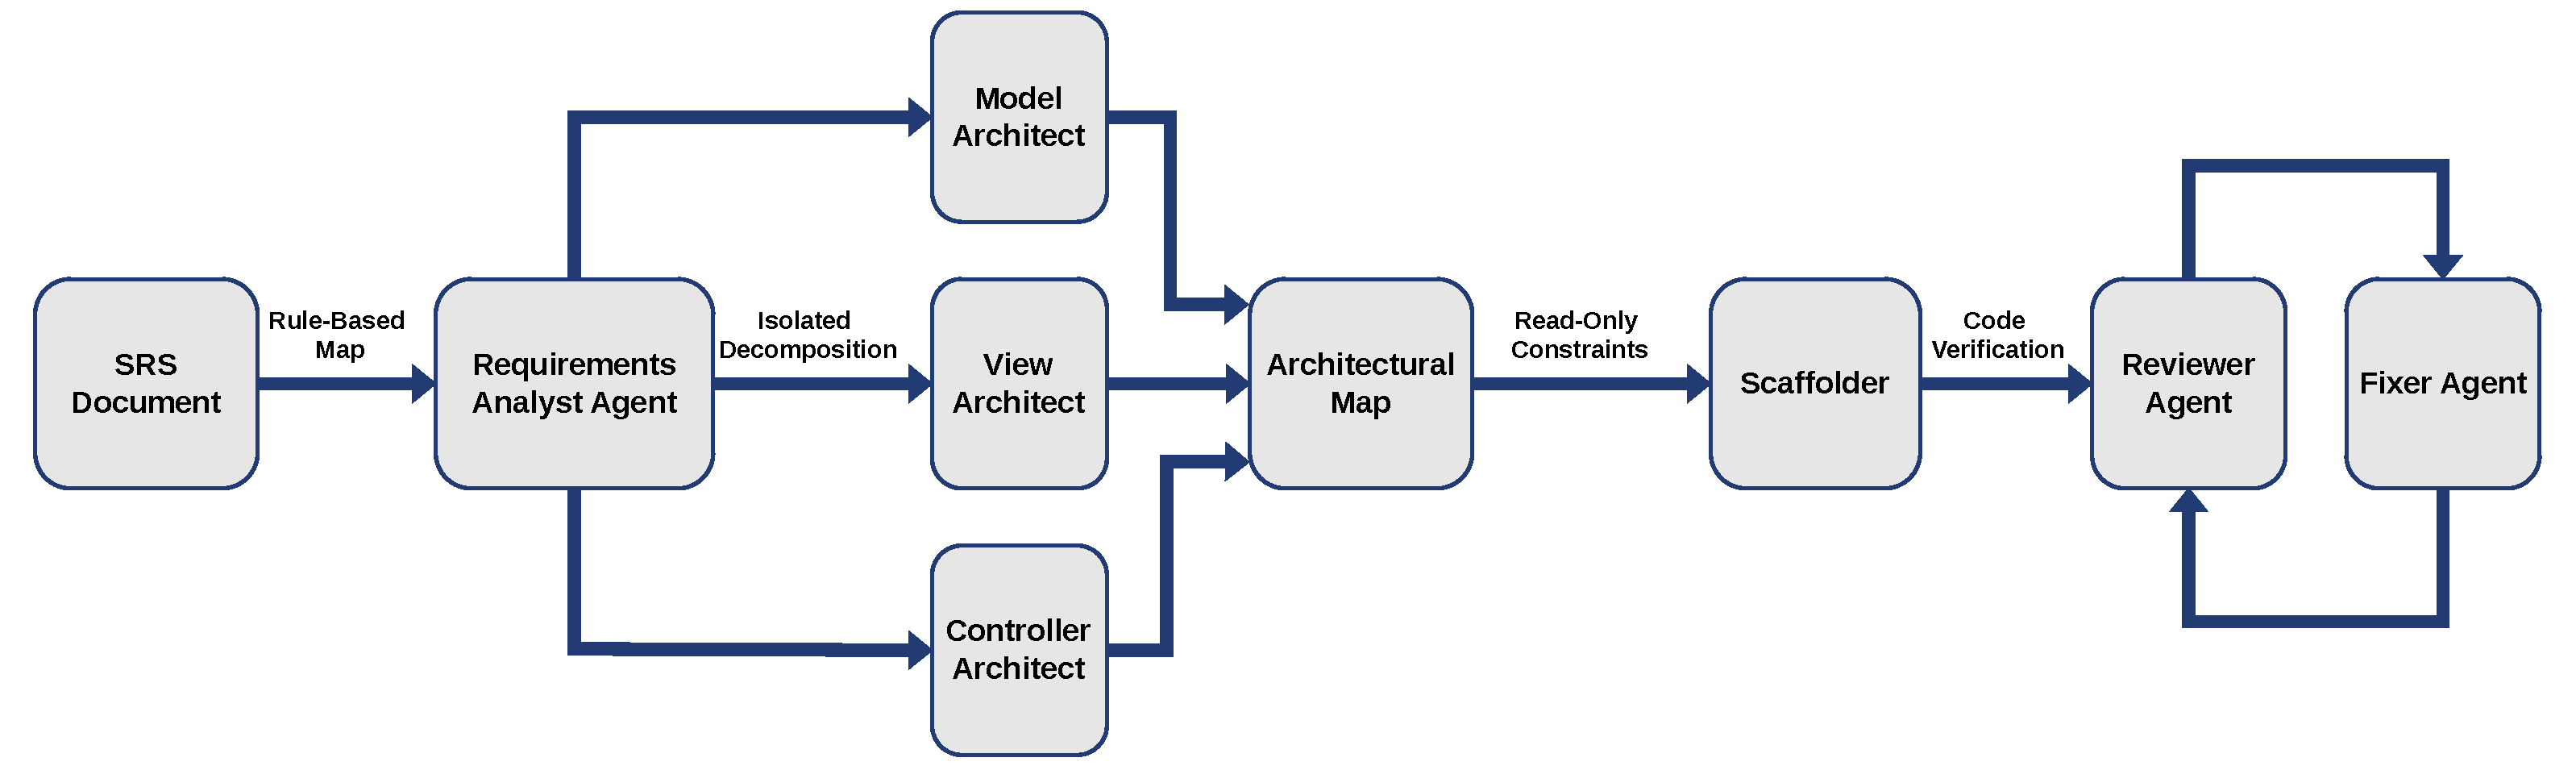
\includegraphics[width=0.80\linewidth]{images/Figure_1.pdf}
\caption{Architecture-First Multi-Agent Orchestration Pipeline. The SRS document is parsed by the Requirements Analyst Agent into a rule-based map, decomposed in isolation by three parallel Architect Agents (Model, View, Controller) into the Architectural Map, and passed as read-only constraints through the rule-based Scaffolder to a verification loop between the Reviewer Agent and Fixer Agent.}
\label{fig:31}
\end{figure}

Operationally, the system is governed by the fundamental ``Separation of Concerns'' principle, implemented through a sophisticated multi-agent topology. Rather than delegating complex, multi-faceted tasks to a single large model, the processes of planning, data extraction, code generation, and verification are decoupled into discrete domains with rigid boundaries. These responsibilities are distributed among highly specialized, independent AI agents. Throughout this paper, the term \textit{agent} refers exclusively to components that invoke an LLM to perform a bounded, task-specific function; the orchestrator, rule-based scaffolder, AST-based static analyzer, and human approval gate operate as rule-based control or analysis components. For instance, while the Requirements Analyst Agent is tasked exclusively with defining the domain taxonomy, the Architect Agents analyze and decompose the Model-View-Controller (MVC) layers in careful isolation. By using this systematic and modular taxonomy, each agent generates outputs constrained solely by its designated area of expertise. This isolation is designed to reduce the margin for hallucination and support the consistency of the generated artifacts under the tested configuration.

Data interoperability within this modular architecture is managed via the JSON format, providing a structured and machine-readable communication channel. This structured payload is designed to ensure that the architectural decisions synthesized by upstream agents serve as constraints for downstream phases. For example, the Architectural Map, generated independently by the Model Architect Agent, View Architect Agent, and Controller Architect Agent, defines the architectural perimeters that the Scaffolder is designed not to breach during code generation. In the final phase, the Reviewer Agent and Fixer Agent operate in tandem to verify that the generated implementation aims to adhere JSON-defined boundaries, autonomously remediating any detected deviations without compromising the initial architectural integrity. This cyclical, multi-agent interaction is designed to combine the stochastic generative capabilities of LLMs with the systematic, rule-based constraints of software engineering, thus establishing a sustainable and architecturally grounded development environment.

The effectiveness of this structured JSON communication protocol, a commonly used grounding strategy for reducing hallucination in LLM outputs, and the enforcement of architectural boundaries depends upon the precise semantic analysis of the initial requirements and their anchoring to a structured knowledge base. The mechanisms by which this critical prerequisite is fulfilled, and the process through which raw natural language data is transformed into structured architectural blueprints, are detailed in the subsequent phase.

\FloatBarrier
\subsection{Phase I: Automating Requirement Extraction: SRS Grounding and Domain Discovery}

The operational workflow for requirement extraction is depicted in Figure~\ref{fig:32}. In classical MVC-based development, the requirements analysis phase is where a human architect reads the specification documents, identifies the domain entities, and maps functional requirements to the Model, View, and Controller layers \citep{Reenskaug1979, Gamma1994}. Phase I automates this exact process. To ground every architectural decision in verified requirements and reduce the risk of hallucination, this phase employs Retrieval-Augmented Generation (RAG) \citep{Lewis2020}: rather than relying on the LLM's parametric knowledge, the system dynamically retrieves only the most semantically relevant SRS segments for each architectural query. Initiated via the \texttt{/extract} command, the operational lifecycle of the system begins with the ``SRS Grounding'' phase, which transforms raw textual inputs into structured, machine-actionable architectural data from which the overall structure of the project is derived.

\begin{figure}[pos=h]
\centering
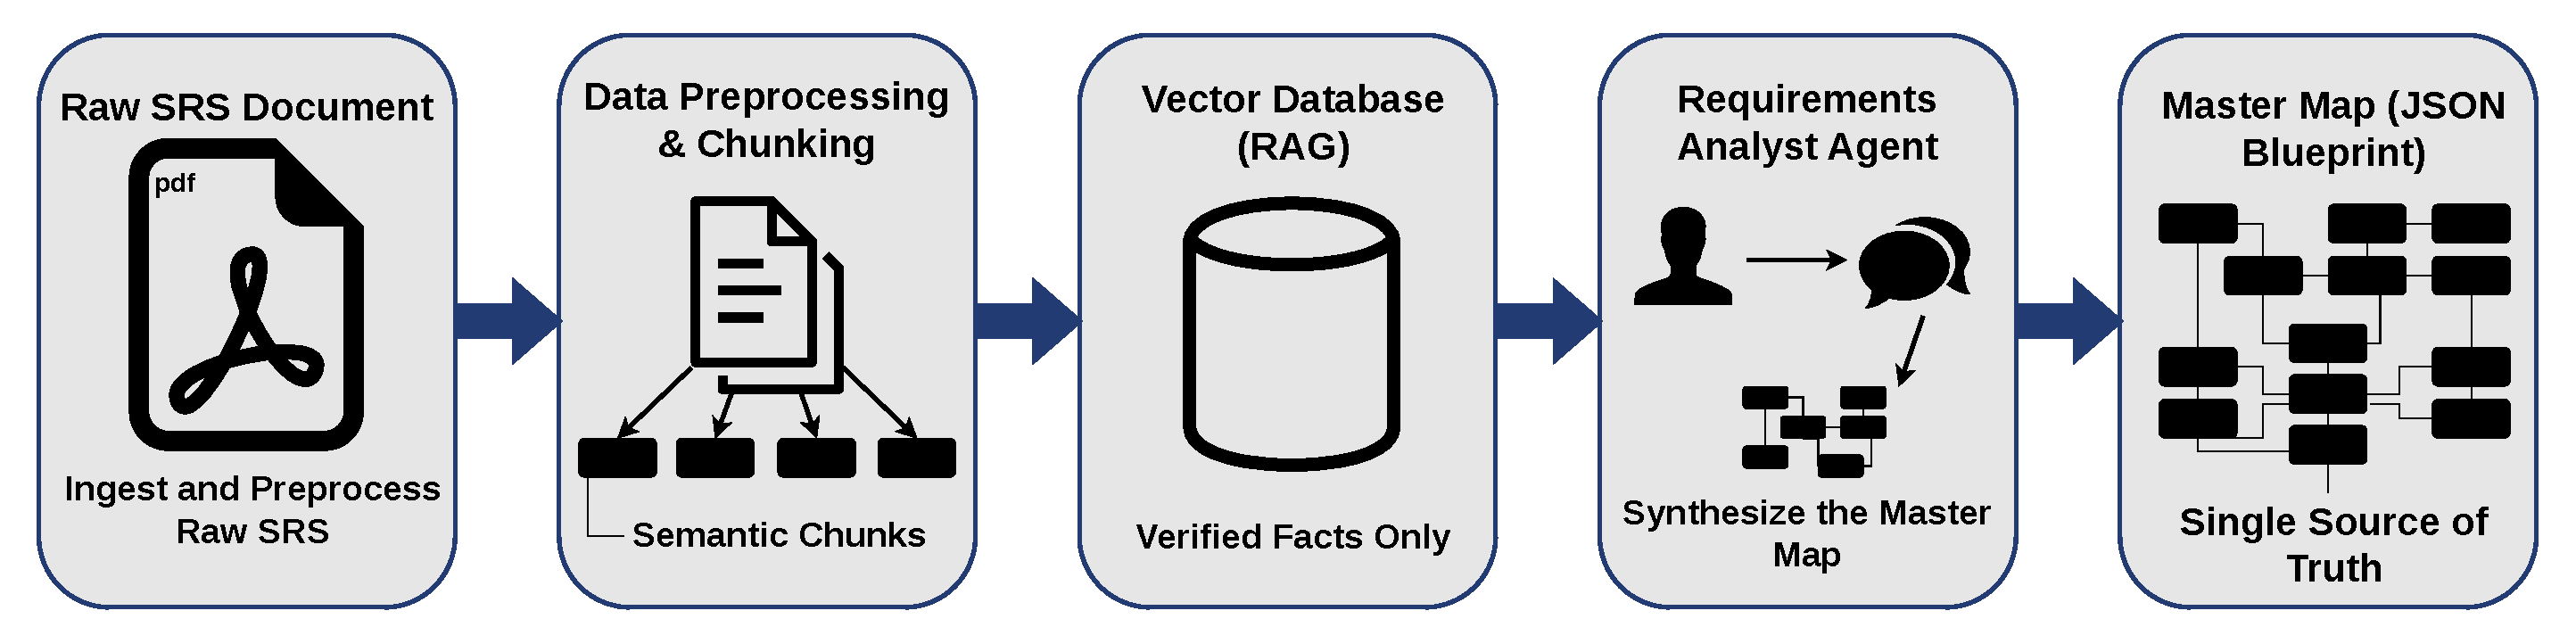
\includegraphics[width=0.80\linewidth]{images/Figure_2.pdf}
\caption{Phase I: SRS Grounding and Domain Discovery workflow. Raw SRS documents are preprocessed into semantic chunks, indexed in a Retrieval-Augmented Generation (RAG) vector database restricted to verified facts, and synthesized by the Requirements Analyst Agent into the Master Map, the system's single source of truth.}
\label{fig:32}
\end{figure}

During initialization, raw SRS documents (typically in PDF format) are ingested into the system. The extracted data undergoes systematic preprocessing to eliminate noise, encompassing format correction, whitespace trimming, and text normalization. The refined text is subsequently partitioned into overlapping segments (chunks) while aiming to preserve semantic integrity. This chunking strategy enables the system to focus exclusively on contextually relevant information blocks during downstream tasks, rather than repeatedly processing the entire document, which is intended to support extraction accuracy while reducing computational overhead.

The sanitized text segments are then embedded and indexed within a vector database, forming the operational core of the Retrieval-Augmented Generation (RAG) strategy. For any given architectural query, the system retrieves only the semantically most relevant SRS segments. By using this vector-based retrieval mechanism, the generative agents are guided to base their architectural synthesis primarily on verified facts. This strategic constraint aims to reduce the injection of fabricated features or hallucinated requirements, ensuring that the generated architectural scaffold remains as faithful as possible to the original specifications.

In the final step of the extraction pipeline, the system derives the Master Map. This artifact represents the formal transformation of complex natural language requirements into a structured ``project constitution'' comprehensible to the AI agents. During this synthesis, the Requirements Analyst Agent evaluates the extracted semantic data to define the foundational framework of the project.

Beyond serving as a high-level conceptual summary, the Master Map functions as a machine-readable, JSON-formatted blueprint detailing the project naming conventions, core data structures (Domain Entities), and primary operational capabilities (System Functions). This blueprint acts as the system's single source of truth. Consequently, all downstream Architect Agents tasked with synthesizing the Model, View, and Controller layers generate their respective class definitions by referencing this centralized map.

This methodology provides a key advantage: it aims to prevent the AI from arbitrarily introducing unnecessary features or unverified logic into the project. Because the functional scope and data constraints are explicitly defined at the project's inception, the system strives to maintain a consistent traceability chain between the initial natural language requirements, the intermediate class structures, and the final source code. This end-to-end traceability promotes consistent and reproducible behavior across all system components throughout the development lifecycle.

Although the Master Map establishes the conceptual foundation of the project, this centralized blueprint is subsequently decomposed in accordance with MVC principles to synthesize a functional software architecture. The subsequent section details how the Model, View, and Controller layers are autonomously constructed in an isolated manner, using this centralized blueprint as their foundational premise.

Large Language Models (LLMs) are used in the extraction phase to overcome semantic ambiguity in SRS documents. Unlike traditional rule-based Natural Language Processing (NLP), which relies on strict syntactic parsing, the LLM acts as a semantic synthesizer. It grasps the broader context to map scattered functional requirements directly into a structured MVC architecture.

In summary, Phase I takes a raw SRS document as input and produces two key outputs: a RAG-indexed vector database of semantically chunked requirements, and the \texttt{requirements\_analysis.json} artifact (Table~\ref{tab:artifact_flow})---a structured JSON blueprint defining the project's domain entities and system functions. This artifact serves as the single source of truth for all downstream agents and is consumed directly by the three Architect Agents in Phase II to decompose the architecture into isolated Model, View, and Controller components.

\FloatBarrier
\subsection{Phase II: Automating Architectural Design: Agent-Driven MVC Component Extraction}
\label{sec:phase2}

The systematic decomposition of the architectural layers is illustrated in Figure~\ref{fig:33}. This phase implements the architectural design process, facilitating the systematic transformation of the Master Map into a concrete Model-View-Controller (MVC) software architecture. The primary objective is to separate abstract architectural reasoning from concrete code generation as cleanly as possible. Consequently, the specifications for each MVC layer are formalized into structured JSON artifacts, bounded by their respective architectural responsibilities. This decomposition is orchestrated by three highly specialized generative agents, the Model, View, and Controller Architect Agents, which aim to enforce the isolation of the system's data structures, presentation layers, and business logic, respectively.

\begin{figure}[pos=h]
\centering
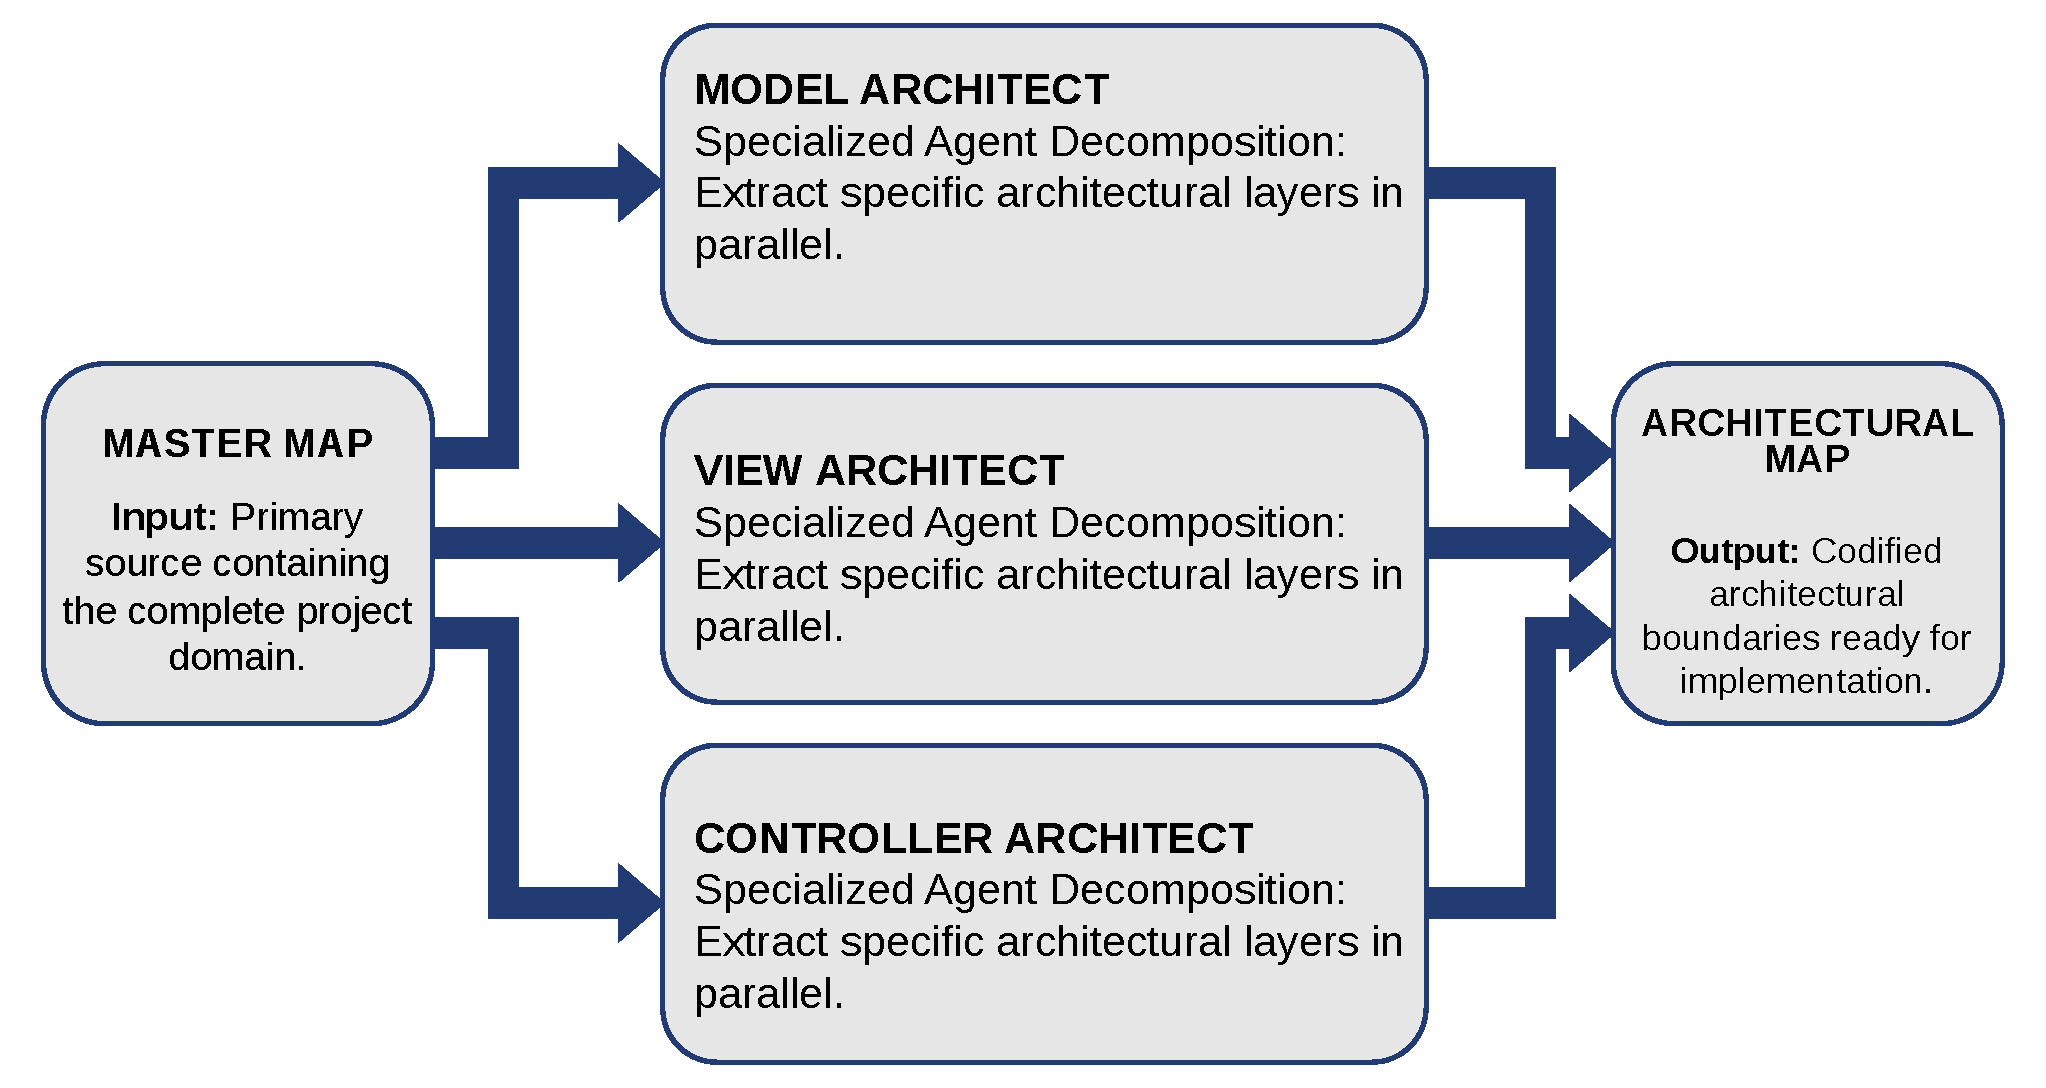
\includegraphics[width=0.80\linewidth]{images/Figure_3.pdf}
\caption{Phase II: Agent-Driven MVC Component Extraction process. The Master Map is decomposed in parallel by three specialized Architect Agents, Model, View, and Controller, each extracting its respective architectural layer, and the resulting outputs are consolidated into the Architectural Map, a structured Model-View-Controller (MVC) JSON artifact ready for implementation.}
\label{fig:33}
\end{figure}

In classical MVC development, formalizing the Model layer is the data architect's responsibility: they manually define domain entities' attributes, data types, and inter-entity relationships, typically through entity-relationship or Unified Modeling Language (UML) class diagrams \citep{Gamma1994}. The Domain Entity Modeling phase automates this exact process. During this phase, the Model Architect Agent autonomously identifies and extracts the core domain entities from the Master Map. To prevent unnecessary complexity and keep the architectural scope manageable, this extraction is capped at a maximum of eight core entities, an implementation limit chosen to bound prompt and artifact size during this feasibility evaluation. These caps are prototype constraints rather than theoretically optimal MVC sizes. Consequently, the system aims to focus the data backbone on the most critical business objects. The resulting JSON artifact explicitly defines the names and functional attributes of each entity, formally establishing the project's semantic data model.

In classical MVC development, the Controller layer is the human architect's responsibility: they manually define which business workflows map to which controller actions, ensuring that the Model and View remain decoupled \citep{Gamma1994}. The Behavioral Logic Mapping phase automates this exact responsibility. Here, the Controller Architect Agent analyzes the documented workflows to synthesize a maximum of six controllers, each constrained to 3–5 specific actions. The most critical constraint enforced during this phase is the ``Zero-Inference'' policy. This heuristic prohibits the agent from autonomously injecting default Create, Read, Update, Delete (CRUD) operations unless they are explicitly mandated by the underlying SRS document. By preventing the generative tendency to hallucinate unnecessary features, this policy aims to preserve architectural fidelity.

Finally, in classical MVC development, the View layer is the interface designer's responsibility: they manually derive the required screens and navigation paths from the documented user journeys \citep{Gamma1994}. The Presentation Layer Abstraction phase automates this exact responsibility, defining the system's interface boundaries. The View Architect Agent synthesizes up to six primary user interfaces based on the extracted user journeys, an implementation limit consistent with the prototype's output-budget constraints, defining solely their functional names and intended purposes. This phase is likewise governed by the ``Zero-Inference'' policy introduced above: the View Architect Agent is prohibited from fabricating screens or interface elements that are not grounded in the extracted user journeys. Crucially, low-level user interface components (e.g., specific buttons, sliders, or graphical widgets) are intentionally abstracted away. This high-level approach allows that the system defines its functional navigation and presentation logic without incurring the overhead of implementation-specific visual details.

In summary, Phase II takes the \texttt{requirements\_analysis.json} artifact produced in Phase I as input and produces the \texttt{architecture\_map.json} artifact (Table~\ref{tab:artifact_flow}), which formally codifies the system's domain entities, controller actions, and user interface boundaries across the three MVC layers. This artifact serves as the architectural constraint for the Scaffolder in Phase III, which translates this abstract design into a concrete, rule-based file system structure.

\FloatBarrier
\subsection{Phase III: Automating Implementation: Rule-Based Scaffolding and Code Generation}
\label{sec:phase3}

In classical MVC development, the implementation phase is where a human developer manually creates the directory structure, writes the class skeletons for each layer, and populates them with business logic, typically guided by the architectural blueprint defined in the design phase \citep{Gamma1994}. Phase III automates this exact workflow through two sequential steps. The transition from architectural abstraction to physical implementation is shown in Figure~\ref{fig:34}. This phase encompasses the implementation stage, wherein the structured JSON artifacts derived in Section~\ref{sec:phase2} are translated into concrete source code. Rather than relying on stochastic, end-to-end code generation, this conversion follows a structured two-step protocol designed to preserve structural integrity. By systematically translating architectural decisions into codebase-level structures, this process aims to reduce the risk of architectural drift between the abstract design and the physical implementation.


The Rule-Based Project Scaffolding step acts as a critical safety perimeter, bridging the abstract architectural blueprint and the concrete file system. Initiated via the \texttt{/scaffold} command, the project's directory hierarchy and foundational class skeletons are synthesized using strict, rule-based algorithms, entirely independent of LLM intervention. This rule-based execution is designed to ensure that all file names, class definitions, and directory trees align with the predefined architectural artifacts. Consequently, structural inconsistencies at the file system level are reduced, providing the developer with a structurally aligned project scaffold intended to support MVC compliance with the SRS.

\begin{figure}[pos=h]
\centering
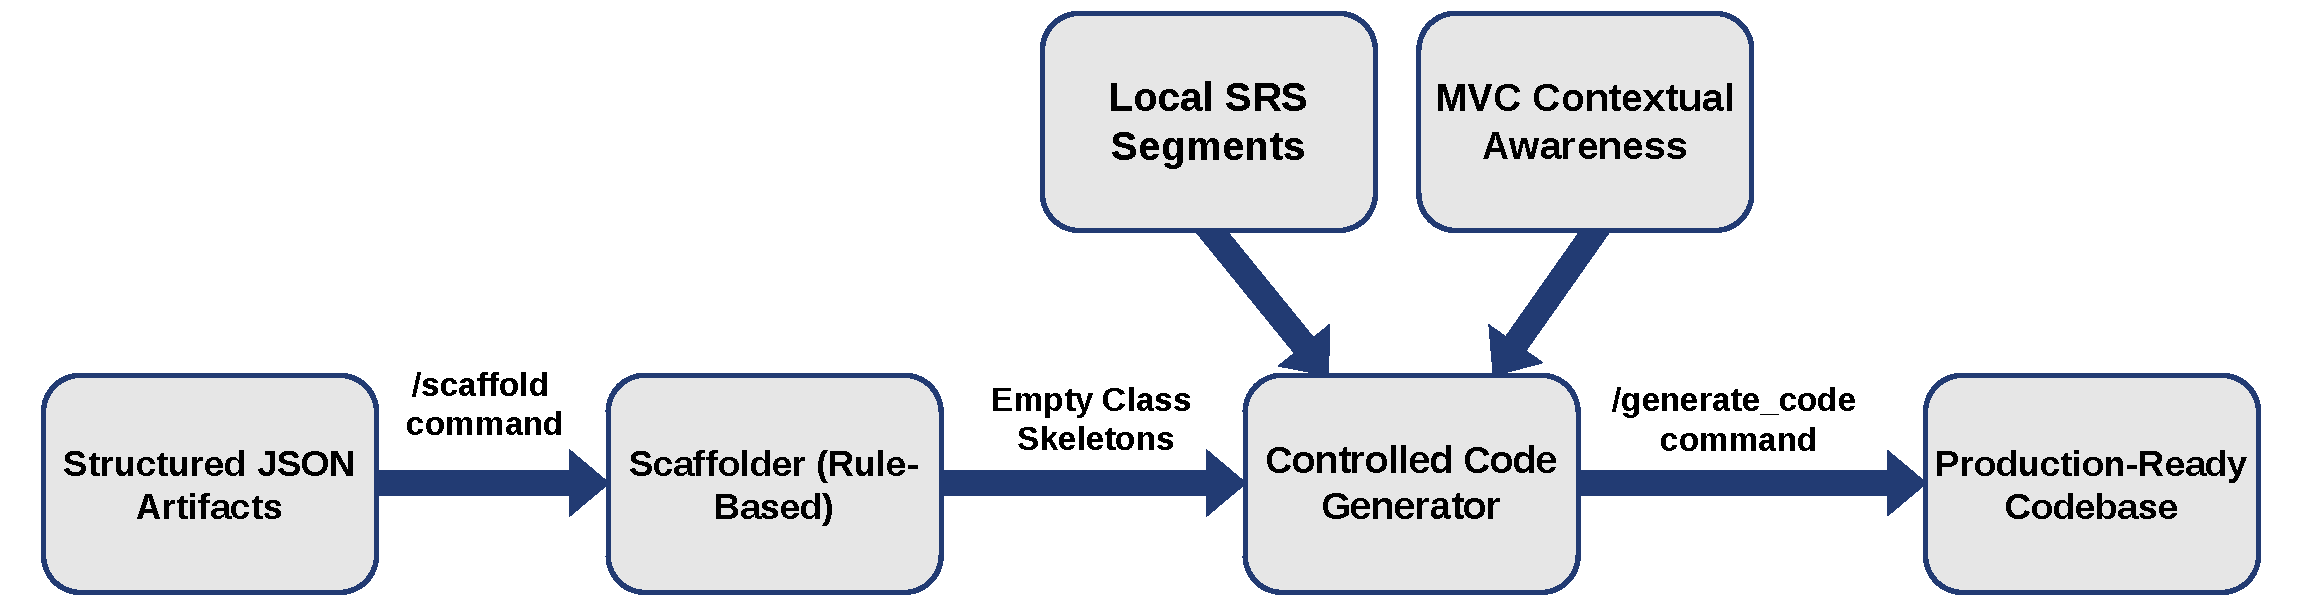
\includegraphics[width=0.80\linewidth]{images/Figure_4.pdf}
\caption{Phase III: Rule-Based Scaffolding and Code Generation workflow. The Structured JSON Artifacts are converted into empty class skeletons by the rule-based Scaffolder via the \texttt{/scaffold} command, which are then populated with Local SRS Segments and MVC Contextual Awareness by the Controlled Code Generator via the \texttt{/generate\_code} command to produce the production-ready codebase.}
\label{fig:34}
\end{figure}

The Code Generation step then populates these empty scaffolds with the actual implementation. Initiated via the \texttt{/generate\_code} command, the developer orchestrates the implementation of specific layers (Model, View, or Controller) by synthesizing contextual data from both the global architectural blueprint and the localized SRS segments. This methodology transitions code generation from a stochastic output model into a highly controlled workflow, tightly constrained by a pre-validated architectural framework.

A critical architectural checkpoint emerges during the generation of the Controller logic. For a controller to orchestrate data flow accurately, it requires contextual awareness of the data it manipulates (Model) and the interfaces it serves (View). To enforce this MVC principle, the code generation pipeline provides the generative agent with explicit, read-only access to these inter-layer relationships, ensuring functional cohesion.

In scenarios where the underlying SRS document exhibits ambiguities or underspecified details, the system is constrained to derive logical inferences solely from the established architectural taxonomy, rather than hallucinating spurious functionalities. By drawing on industry-standard ``reasonable defaults,'' the system synthesizes the missing business logic in a manner that remains consistent with the project's overarching architectural intent.

In summary, Phase III takes the \texttt{architecture\_map.json} artifact from Phase II (Table~\ref{tab:artifact_flow}) as input and produces two outputs: a rule-based project scaffold defining the directory structure and class skeletons, and an LLM-generated implementation constrained by the Architectural Map and SRS segments. The resulting codebase targets Python engineering standards (e.g., PEP 8) and static typing, aiming to provide a structured and maintainable foundation. However, since LLM-based generation is inherently stochastic, the generated code is passed directly to Phase IV, where it is audited for MVC compliance and any detected violations are autonomously remediated.

\subsection{Phase IV: Automating Code Review: MVC-Based Auditing and Autonomous Remediation Loop}

In classical MVC development, ensuring that an implementation respects layer boundaries is the human reviewer's responsibility: code review is where violations such as a View directly accessing a Model are caught before integration \citep{Gamma1994}. Phase IV automates this exact responsibility, extended in this study to include violation categories specific to this system's Controller-centric design, such as business logic displaced outside the Controller (Section~\ref{sec:experiment}). The autonomous verification and remediation cycle is illustrated in Figure~\ref{fig:35}. This phase, characterized by autonomous error detection and self-healing capabilities, represents one of the principal contributions of the \textit{MVC Test Orchestrator}. Beyond generating architecturally compliant scaffolds and implementations, the system continuously monitors the codebase for adherence to the predefined architectural constraints. By filtering stochastic LLM outputs through a rule-based validation mechanism, this phase detects and repairs selected MVC layer violations in the generated artifacts.

\begin{figure}[pos=h]
\centering
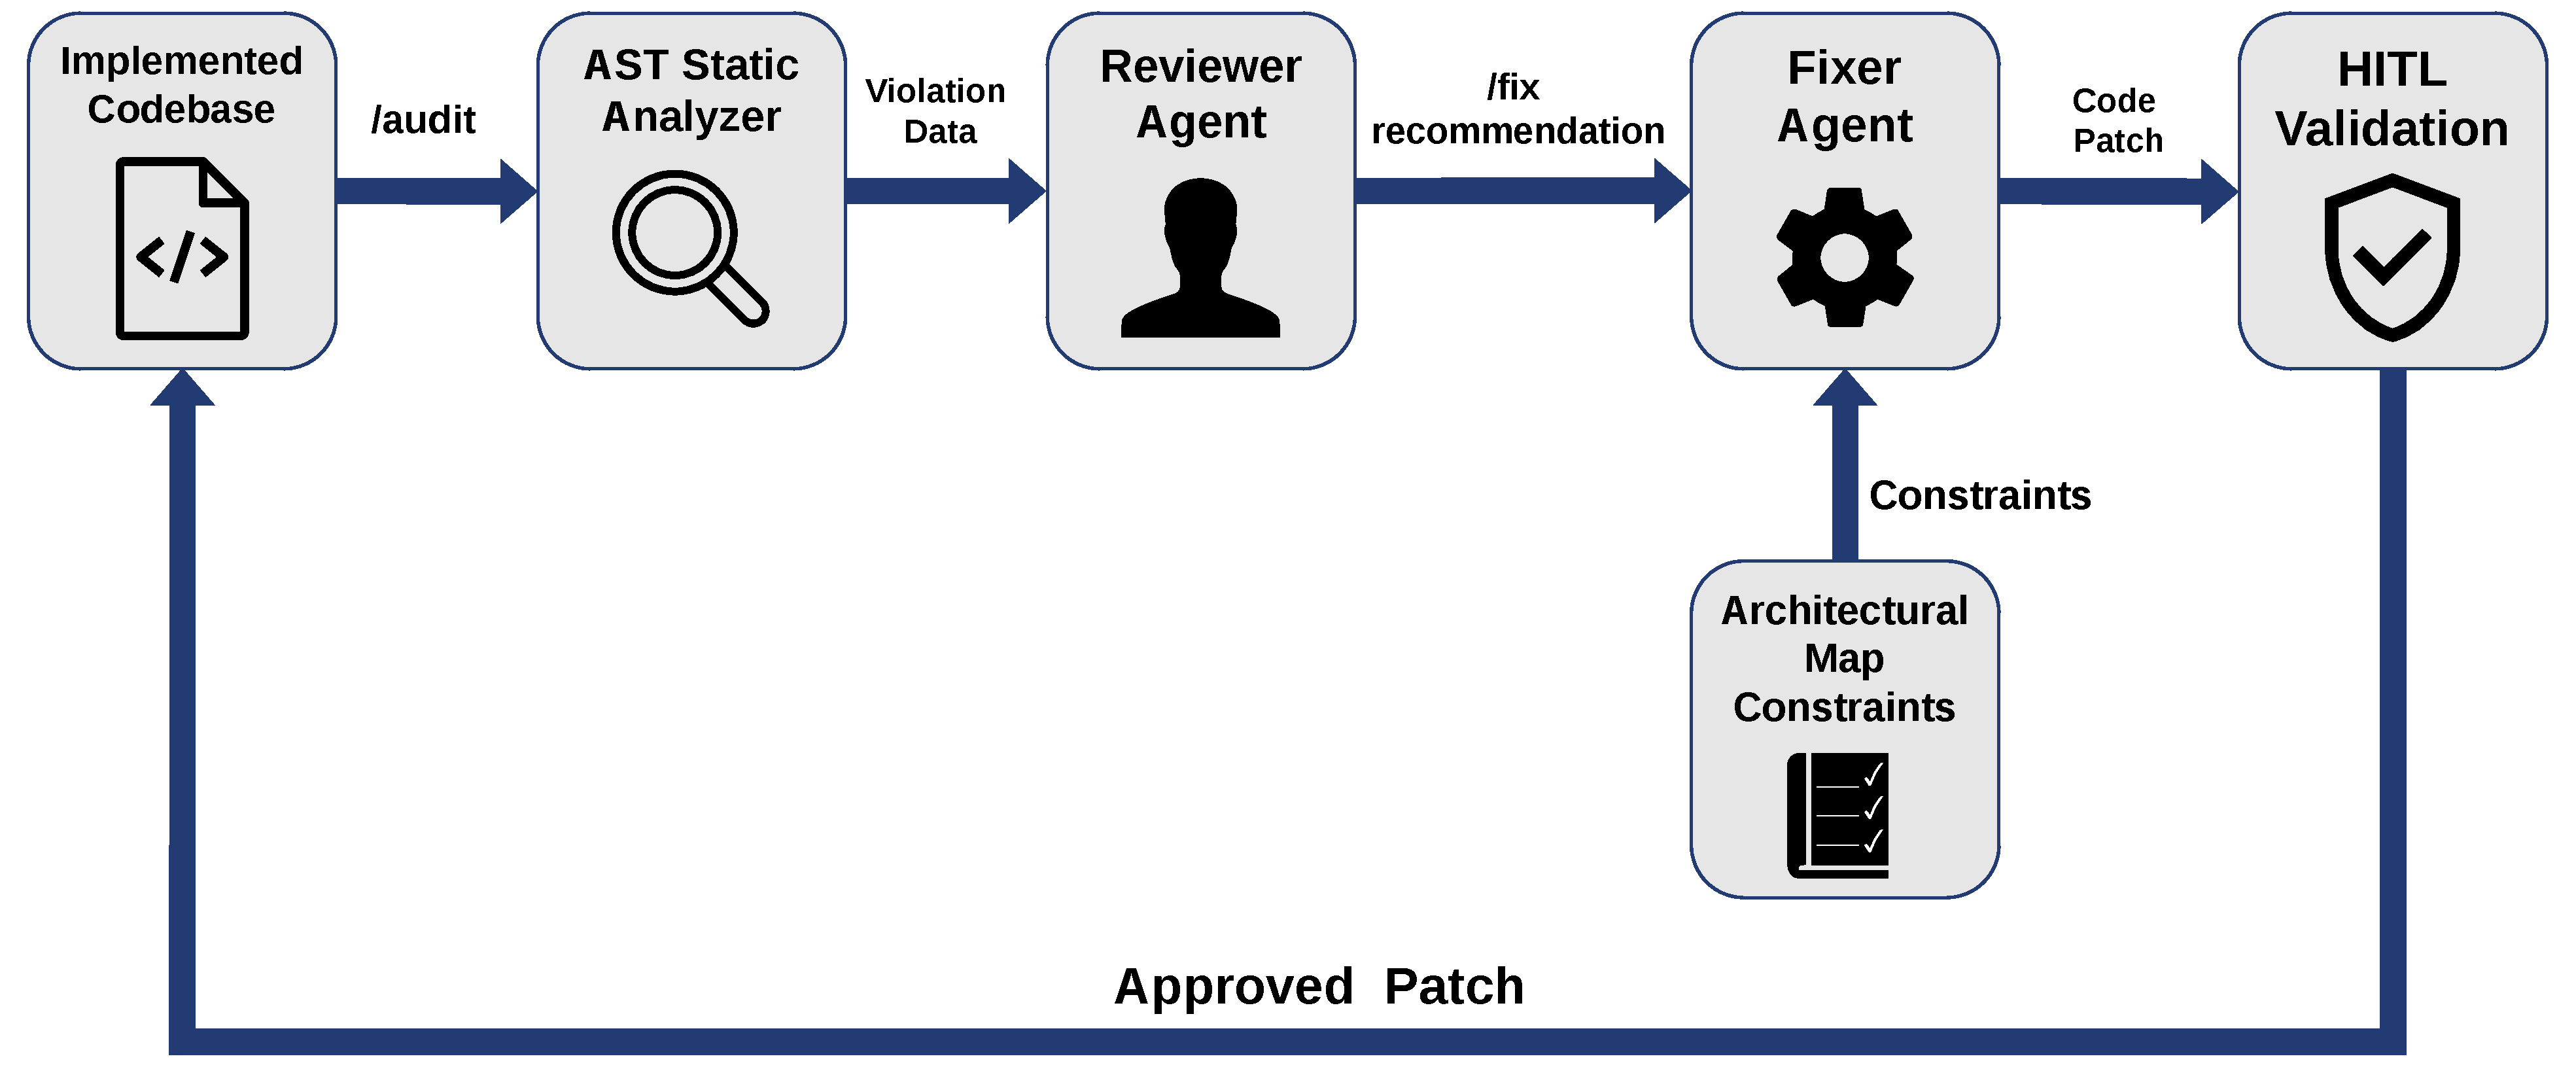
\includegraphics[width=0.80\linewidth]{images/Figure_5.pdf}
\caption{Phase IV: Automated Auditing and Self-Healing Loop. The implemented codebase is inspected by the Abstract Syntax Tree (AST) Static Analyzer via the \texttt{/audit} command, whose violation data is triaged by the Reviewer Agent; the Fixer Agent then patches the code under Architectural Map constraints via the \texttt{/fix} recommendation, subject to Human-in-the-Loop (HITL) validation before the approved patch returns to the codebase.}
\label{fig:35}
\end{figure}

The core of this validation mechanism is a rule-based static analysis framework built upon Abstract Syntax Tree (AST) parsing. Triggered via the \texttt{/audit} command, this module comprehensively inspects the implemented codebase, verifying both syntactic validity and adherence to inter-layer dependency constraints. For instance, MVC isolation violations, such as a View component directly instantiating or querying a Model object, are statically detected prior to execution. The analyzer implements four bounded, syntax-directed checks over Python ASTs combined with pattern-based rules; it is not a general semantic defect detector.

Detected violations are aggregated into a structured, machine-readable feedback report, which the Reviewer Agent uses to synthesize concrete, actionable refactoring strategies to resolve the identified violations.

The culmination of the validation process is the constrained remediation phase, initiated via the \texttt{/fix} command. Operating on the telemetry provided by the \texttt{/audit} report, the Fixer Agent autonomously patches the defective code blocks while aiming to preserve architectural integrity. This remediation is explicitly ``constrained'' because the generative agent treats the Architectural Map and the rule-based project scaffold as read-only, restricting its edits to the flagged code blocks alone. This limitation minimizes the risk of introducing secondary structural regressions while resolving an isolated bug. Ultimately, the \texttt{/fix} mechanism integrates automated repair with a Human-in-the-Loop (HITL) protocol, requiring developer validation before committing the proposed architectural patches.

In summary, Phase IV takes the generated codebase from Phase III as input and produces two outputs: the \texttt{violations.json} artifact (Table~\ref{tab:artifact_flow}) detailing all detected MVC layer breaches, and a patched codebase in which identified violations have been autonomously remediated by the Fixer Agent within the boundaries of the \texttt{architecture\_map.json} artifact. The patched code is then presented to the developer for final validation through the HITL protocol, which governs the strategic oversight of all four phases and is described in the following subsection.


\subsection{Human-in-the-Loop (HITL) Integration}

The balanced interaction between human expertise and automated processes is depicted in Figure~\ref{fig:36}. The proposed methodology embeds human strategic governance into the generative loop. Rather than functioning as an opaque, fully autonomous black-box, the \textit{MVC Test Orchestrator} implements a structured Human-in-the-Loop (HITL) paradigm. This architecture formalizes an iterative control mechanism between the developer and the multi-agent system. At its core, this approach provides checkpoints at which a developer may inspect, reject, or edit intermediate artifacts before the pipeline advances, offering a mechanism to align the generative throughput of LLMs with the strategic oversight and judgment of human software engineers.

\begin{figure}[pos=h]
\centering
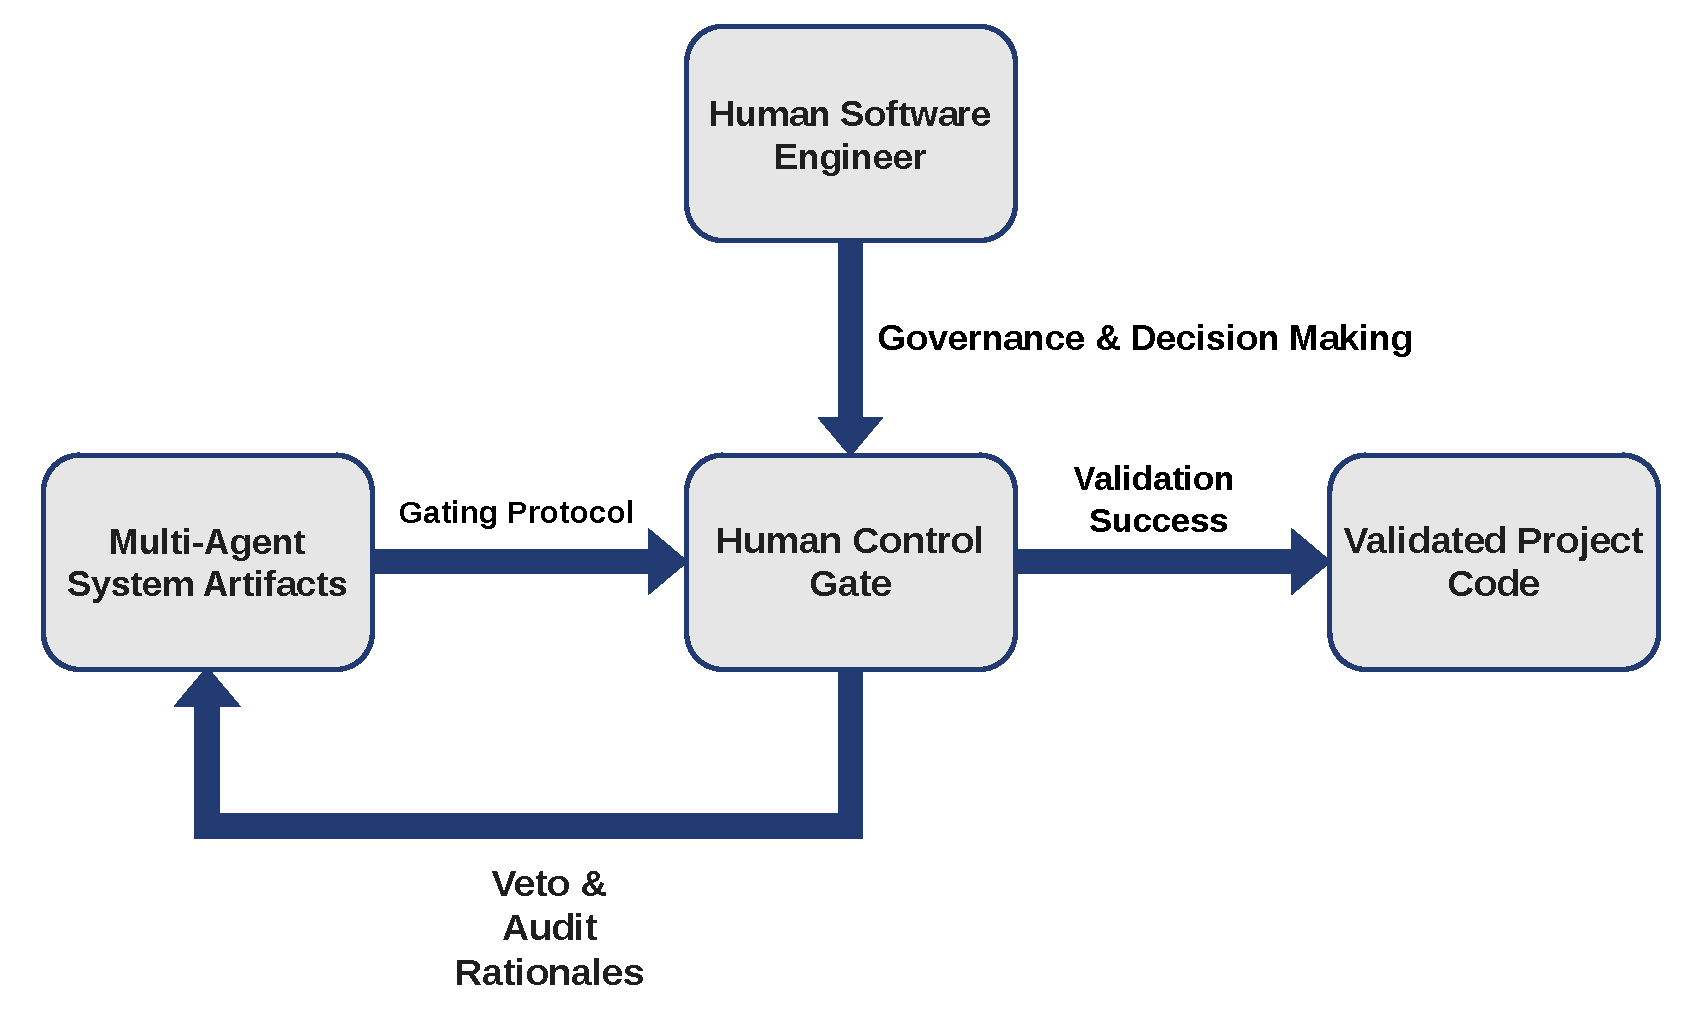
\includegraphics[width=0.62\linewidth]{images/Figure_6.pdf}
\caption{Strategic Human-in-the-Loop Governance Protocol. The Human Software Engineer exercises governance over the Human Control Gate, which admits Multi-Agent System Artifacts through a gating protocol and either validates them into approved project code or returns veto and audit rationales back to the artifacts for revision.}
\label{fig:36}
\end{figure}

The HITL mechanism acts as a structured gating protocol at critical points within the pipeline. The developer retains the authority to inspect, modify, or veto the system's outputs at every phase, from the initial JSON-based architectural scaffolding to the final AST-driven code review. Furthermore, the explainable, natural-language rationales generated during the \texttt{/audit} and \texttt{/fix} phases equip developers with the necessary context to objectively evaluate the AI's technical recommendations. By bounding AI autonomy within this collaborative framework, the system helps reduce cascading structural errors within the generated codebase. Ultimately, preserving developer sovereignty over the project supports a development lifecycle that is both architecturally resilient and industrially viable.

\subsection{Inter-Phase Artifact Summary}

Each pipeline phase produces a structured, machine-readable artifact that serves as the sole communication contract between successive agents. Table~\ref{tab:artifact_flow} consolidates these artifacts: the phase in which each is generated (with a reference to the corresponding workflow figure), its contents, and the downstream component that consumes it. This table is used as the unified reference throughout Section~\ref{sec:experiment} and Section~\ref{sec:results}, replacing repeated inline file-name citations.

% --- ARTIFACT FLOW TABLE ---
\begin{table}[pos=h]
\centering
\caption{Inter-phase artifact flow: structured outputs generated and consumed across pipeline phases.}
\label{tab:artifact_flow}
\renewcommand{\arraystretch}{1.3}
\begin{tabularx}{\textwidth}{@{} >{\raggedright\arraybackslash}X l >{\raggedright\arraybackslash}X >{\raggedright\arraybackslash}X @{}}
\toprule
\textbf{Artifact (File Name)} & \textbf{Generated In} & \textbf{Contents} & \textbf{Used In} \\
\midrule
Requirements Analysis Artifact \newline (\texttt{requirements\_analysis.json}) & Phase I (Fig.~\ref{fig:32}) & Extracted domain entities and system functions synthesized from the SRS by the Requirements Analyst Agent & Phase II --- Architect Agents \\
\midrule
Architectural Map Artifact \newline (\texttt{architecture\_map.json}) & Phase II (Fig.~\ref{fig:33}) & MVC component definitions (Model, View, Controller) produced by the three Architect Agents & Phase III --- Scaffolder \\
\midrule
Scaffolded Codebase Artifact & Phase III (Fig.~\ref{fig:34}) & MVC directory structure with class skeletons and template files generated systematically from \texttt{architecture\_map.json} & Phase IV --- AST-based static analyzer \\
\midrule
Violation Report Artifact \newline (\texttt{violations.json}) & Phase IV (Fig.~\ref{fig:35}) & Detected architectural violations with severity levels produced by the AST-based static analyzer & Phase IV --- Fixer Agent \\
\bottomrule
\end{tabularx}
\end{table}
\section{Experiments}
\label{sec:experiment}

Following the detailed exposition of the \textit{MVC Test Orchestrator}'s multi-agent architecture, RAG-driven knowledge extraction, and structured control mechanisms in Section~\ref{sec:methodology}, this section presents an experimental evaluation of the system's performance across 20 distinct SRS documents.

\subsection{Research Questions and Experiment Design}

The evaluation is structured around five core Research Questions (RQs) that collectively assess the framework's architectural extraction score, layered compliance enforcement, autonomous remediation effectiveness, human-AI agreement, and stochastic output consistency:

\begin{itemize}
    \item \textbf{RQ1 (Architectural Extraction Score):} To what extent can the system accurately isolate Model, View, and Controller components from unstructured, raw SRS documents?
    \item \textbf{RQ2 (Layered Compliance):} To what degree does the proposed multi-agent architecture preserve the separation of concerns and enforce isolation between MVC layers?
    \item \textbf{RQ3 (Remediation Effectiveness):} How effective is the Constrained Remediation Phase in rectifying identified architectural violations while maintaining fidelity to the original requirements?
    \item \textbf{RQ4 (Human-AI Agreement):} To what extent are the autonomously generated architectural designs deemed accurate, sufficient, and industrially viable by expert software engineers?
    \item \textbf{RQ5 (Consistency and Reliability):} What is the system's stochastic variance and output consistency when subjected to identical inputs across multiple iterations?
\end{itemize}

The experiments were conducted on a corpus of 20 distinct SRS documents. These documents constitute a purposive, criterion-based sample drawn from high-performing senior-level software engineering capstone projects at one institution, all of which were evaluated by an academic committee and received scores of 90/100 or higher. The 90/100 threshold was applied to reduce noise from severely incomplete specifications, not to construct a representative sample of industrial SRS practice. While a corpus of this size is appropriate for an expert-validated qualitative evaluation, it remains modest for drawing strong statistical generalizations about system performance. This selection substantially expands upon the five initial cases presented in our preliminary work \citep{dim2026mvc}. The descriptive metadata for these SRS documents is provided
in Table~\ref{tab:srs_dataset}.

For each experimental scenario, the system executed the complete operational workflow: requirement synthesis
(Phase I), architectural design inference (Phase II), rule-based scaffolding (Phase III), and code generation coupled
with AST-based verification (Phase IV). To quantify the system’s ability to constrain stochastic LLM variance
(RQ5), the architectural derivation phase was repeated three times for each SRS using identical model parameters
(temperature, top-p) and prompts. A Consistency Score was subsequently calculated by comparing the component name sets produced across the three independent runs using a set-intersection-based consistency metric (Eq.~\ref{eq:cs}).
To objectively evaluate the human-AI agreement and populate the Architectural Component Extraction Score (ACES), a validation protocol was implemented in which expert software engineers evaluated the autonomously generated MVC components using a structured, multi-dimensional Evaluation Rubric. The HITL checkpoints were available at each phase boundary but were not exercised during these experiments; the pipeline was executed in fully automated mode to isolate the system's autonomous capabilities. Accordingly, this study does not estimate the effect of human intervention on output quality, time, or acceptance.

% --- DATASET TABLE ---
\begin{table}[pos=h]
\centering
\caption{Descriptive metadata of the 20 Software Requirements Specification (SRS) documents used in the experiments.}
\label{tab:srs_dataset}
\begin{tabular}{llcccc}
\toprule
\textbf{SRS ID} & \textbf{SRS Title} & \textbf{Pages} & \textbf{Characters} & \textbf{Tokens} & \textbf{Requirements} \\
\midrule
SRS \#1  & Online Rent a Car                             & 26 & 33384 & 6518  & 62 \\
SRS \#2  & Human Resources Management System             & 47 & 73860 & 14724 & 71 \\
SRS \#3  & Online Tourist Guide                          & 24 & 26162 & 4776  & 24 \\
SRS \#4  & Crime and Criminal Intelligence System        & 21 & 29348 & 5562  & 40 \\
SRS \#5  & Pet Hotel Reservation System                  & 33 & 45631 & 8830  & 39 \\
SRS \#6  & Online Cargo Tracking System                  & 20 & 23195 & 3990  & 42 \\
SRS \#7  & Social Network System                         & 23 & 37681 & 8166  & 38 \\
SRS \#8  & Online Diet Consultancy                       & 23 & 35783 & 6631  & 39 \\
SRS \#9  & Temperature Control System                    & 30 & 47123 & 9052  & 40 \\
SRS \#10 & Hospital Management System                    & 37 & 35521 & 6898  & 40 \\
SRS \#11 & Online Airline Reservation System             & 25 & 37423 & 7548  & 40 \\
SRS \#12 & Online Legal Advisor System                   & 14 & 21904 & 4017  & 27 \\
SRS \#13 & Restaurant Reservation                        & 25 & 39559 & 7481  & 35 \\
SRS \#14 & Chat Application                              & 35 & 40113 & 7880  & 31 \\
SRS \#15 & Fingerprint Voting System                     & 25 & 31282 & 6135  & 23 \\
SRS \#16 & Pharmacy Management System                    & 23 & 31869 & 6100  & 31 \\
SRS \#17 & Smart Home Management System                  & 22 & 37579 & 7679  & 27 \\
SRS \#18 & Railway Tracking and Arrival Time Prediction  & 24 & 22285 & 4802  & 23 \\
SRS \#19 & Hotel Management System                       & 31 & 44754 & 8435  & 40 \\
SRS \#20 & Online Shopping Site                          & 39 & 50553 & 10150 & 31 \\
\bottomrule
\end{tabular}
\end{table}

\subsection{Implementation Environment}

All experiments were conducted using \textit{Gemini 2.5 Flash},
accessed via the Google Generative AI API~\citep{gemini2025}, as the underlying
large language model. The multi-agent orchestration pipeline was 
implemented in Python, utilizing the Google Generative AI 
SDK~\citep{googlegenai2025} for LLM interactions, Python's 
built-in \texttt{ast} module for AST-based static analysis, and 
the \texttt{bert\_score} library~\citep{zhang2019bertscore} for 
semantic consistency evaluation. All agents operated on identical 
prompts and model hyperparameters across experimental runs to 
support reproducibility. Given identical SRS input, model 
parameters, and prompts, the pipeline is expected to produce 
consistent \texttt{requirements\_analysis.json} and 
\texttt{architecture\_map.json} artifacts, as quantified by the 
Consistency Score metric (Eq.~\ref{eq:cs}). The 
rule-based scaffolding and AST-based auditing phases do not involve
LLM inference and are expected to produce consistent outputs across
repeated runs.
The source code of the \textit{MVC Test Orchestrator} pipeline
is publicly available~\citep{mvctestorchestrator2026}.

Table~\ref{tab:reproducibility} consolidates the configuration parameters required to reproduce the reported experiments.

\begin{table}[htbp]
\centering
\caption{Reproducibility configuration. Pipeline parameters are sourced directly from \texttt{core/config.py} in the public repository~\citep{mvctestorchestrator2026}; BERTScore evaluation parameters are reported below for methodological transparency.}
\label{tab:reproducibility}
\renewcommand{\arraystretch}{1.2}
\begin{tabularx}{\textwidth}{@{} l >{\raggedright\arraybackslash}X @{}}
\toprule
\textbf{Parameter} & \textbf{Value} \\
\midrule
LLM model identifier     & \texttt{gemini-2.5-flash} \\
Embedding model          & \texttt{distiluse-base-multilingual-cased-v1} \\
Chunk size               & 1{,}000 characters \\
Chunk overlap            & 100 characters \\
Retrieval top-\textit{k} & 5 \\
Vector store collection  & \texttt{srs\_collection} (user-provided) \\
BERTScore model          & \texttt{roberta-large} (\texttt{lang=`en'}) \\
BERTScore settings       & \texttt{rescale\_with\_baseline=False}, \texttt{idf=False} \\
BERTScore component reported & F1 \\
\bottomrule
\end{tabularx}
\end{table}

\subsection{Evaluation Metrics and Validation Protocol}

The metrics used to evaluate the system's effectiveness go beyond traditional code generation accuracy; they are specifically engineered to quantify the quality of data transformation at every critical juncture, from raw requirements to the executable codebase. The evaluation process employs the following metrics, each grounded in the system's input-output pipeline. The numerical results yielded by each metric across all 20 SRS documents are consolidated in Table~\ref{tab:end_to_end_performance} (Section~\ref{sec:results}); the subsections below formally define each metric, state its directional interpretation with respect to the corresponding RQ, and link it to the relevant pipeline artifact (Table~\ref{tab:artifact_flow}). A consolidated metric-to-RQ interpretation is also provided in Table~\ref{tab:metric_rq_mapping} at the end of this section.

As detailed in Table~\ref{tab:artifact_flow} (Section~\ref{sec:methodology}), each pipeline phase produces a structured artifact that coordinates agent communication. The metric definitions below refer to that table rather than restating individual file names inline.

\subsubsection{Semantic Consistency and Extraction Score (RQ1 \& RQ4)}

To objectively measure the system's ability to isolate architectural components from unstructured text, two complementary metrics are employed: BERTScore for semantic analysis and ACES for expert validation.

\textbf{Semantic Consistency of Requirements (BERTScore):} As described in Phase I (Fig.~\ref{fig:32}), the SRS Grounding stage produces the Requirements Analysis Artifact (Table~\ref{tab:artifact_flow}), which encapsulates the functional requirements autonomously extracted by the LLM. This metric quantifies the semantic overlap between that artifact and the original functional specifications within the raw SRS document. Deviating from traditional, inflexible ``exact-match'' or n-gram methodologies, this evaluation prioritizes semantic fidelity using BERTScore~\citep{zhang2019bertscore} (configuration reported in Table~\ref{tab:reproducibility}). Each extracted requirement (domain entity or system function) in the Requirements Analysis Artifact was treated as an individual candidate string and compared against the SRS document's paragraphs (segmented on blank lines, with fragments under five words excluded) as reference strings; for each candidate, the maximum-scoring reference paragraph was retained, and the per-SRS BERTScore was obtained by averaging across all extracted requirements for that document. BERTScore does not establish requirement completeness or the absence of hallucinated components; these constructs would require requirement-level gold annotations.

\textbf{Architectural Component Extraction Score (ACES):} As described in Phase II (Fig.~\ref{fig:33}), the Architect Agents produce the Architectural Map Artifact (Table~\ref{tab:artifact_flow}), which is subjected to rigorous peer review by a panel of five expert software engineers. Relying on the original SRS documents as the baseline truth, the experts evaluate the autonomously extracted components. To ensure objective and standardized scoring, evaluations are conducted using a structured 0-5 Likert-scale rubric, detailed in Table~\ref{tab:evaluation_rubric}.

% --- MASTER RUBRIC TABLE ---
\begin{table}[pos=h]
\centering
\caption{The structured evaluation rubric used by expert software engineers to assess Model, Controller, and View Extraction Score.}
\label{tab:evaluation_rubric}
\renewcommand{\arraystretch}{1.3} 
\begin{tabularx}{\textwidth}{@{} l >{\raggedright\arraybackslash}X c @{}}
\toprule
\textbf{Metric / Criterion} & \textbf{Description} & \textbf{Scale} \\
\midrule
\multicolumn{3}{@{}l}{\textbf{Model Extraction Score (MES):} Ability to isolate data structures and domain entities.} \\
\midrule
Entity Extraction & Identification of all core actors and objects (e.g., User, Order) from the SRS. & 0-5 \\
Attribute Accuracy & Alignment of model fields and data types with the documented requirements. & 0-5 \\
Relationship Logic & Logical establishment of relational dependencies (1-N, N-M) between models. & 0-5 \\
Naming Consistency & Adherence of nomenclature to SRS terminology and technical standards (e.g., PEP 8). & 0-5 \\
\midrule
\multicolumn{3}{@{}l}{\textbf{Controller Extraction Score (CES):} Ability to manage business logic and coordination.} \\
\midrule
Action Definition & Accurate translation of SRS workflows into specific controller actions (e.g., Create, List). & 0-5 \\
M-V-C Linkage & Correct orchestration between Model data utilization and View redirection. & 0-5 \\
Separation of Concerns & Clear isolation of business logic within the Controller, preventing layer leakage. & 0-5 \\
Functional Completeness & Exhaustive representation of core business workflows (critical paths) as actions. & 0-5 \\
\midrule
\multicolumn{3}{@{}l}{\textbf{View Extraction Score (VES):} Ability to abstract user touchpoints and presentation logic.} \\
\midrule
Screen Coverage & Comprehensive definition of all primary interfaces mentioned in the SRS (e.g., Dashboard). & 0-5 \\
User Journey Alignment & Congruence of the screen hierarchy with the documented user stories/steps. & 0-5 \\
Abstraction Level & Appropriate functional abstraction without being burdened by unnecessary visual details. & 0-5 \\
Hallucination Control & Adherence to the Zero-Inference policy; no fabricated screens or components. & 0-5 \\
\bottomrule
\end{tabularx}
\end{table}

\textbf{Mathematical Formulation of Extraction Scores:} Rather than calculating disjointed averages, the final component score ($Score_{final}$) for each MVC layer---Model Extraction Score (MES), Controller Extraction Score (CES), and View Extraction Score (VES), as defined in Table~\ref{tab:evaluation_rubric}---is formally derived using a two-step aggregation. First, the mean score for a specific layer is calculated for each expert ($E_j$) based on the four underlying criteria ($C_i$). Subsequently, the overall score is determined by averaging the scores across all five experts ($N=5$), as formalized in Equation~\ref{eq:accuracy_score}:

\begin{equation} \label{eq:accuracy_score}
Score_{final} = \frac{1}{4N} \sum_{j=1}^{N} \sum_{i=1}^{4} C_{i,j}
\end{equation}

Where $C_{i,j} \in [0, 5]$ represents the score assigned to the $i$-th criterion by the $j$-th expert. For readability alongside the study's other percentage-based metrics, $Score_{final}$ is additionally reported on a 0--100 scale as $(Score_{final}/5) \times 100$; this rescaled value, rather than a proportion of successful outcomes, is what is reported as ``ACES'' throughout this paper (e.g., 74.0\% corresponds to $Score_{final} = 3.70$). A high $Score_{final}$ (approaching 5) indicates that the system accurately extracts the corresponding MVC components from the SRS, providing a positive answer to \textbf{RQ1}. Conversely, a low score reveals systematic extraction failures in that layer. \textbf{RQ4} is addressed separately, through the inter-rater reliability of the five experts' scores rather than the score magnitude itself (Section~\ref{sec:discussion_rq4}): high agreement among experts supports the reliability of the ACES scores as a valid measure of industrial viability, whereas low agreement would undermine confidence in that interpretation. The aggregate BERTScore and ACES values across all 20 SRS documents are reported in the first two rows of Table~\ref{tab:end_to_end_performance}.

\subsubsection{Enforcement of Layered Compliance (RQ2)}

To determine if the multi-agent architecture preserves the separation of concerns (RQ2), the system's structural integrity is measured through scaffolding precision and static violation detection.

\textbf{Scaffolder Error Rate (SER):} As described in Phase III (Fig.~\ref{fig:34}), the Scaffolder consumes the Architectural Map Artifact (Table~\ref{tab:artifact_flow}) and translates it into a concrete physical directory structure. SER functions as a scaffold transformation integrity check rather than evidence of generative accuracy: it verifies that the rule-based translation produced no missing, misnamed, or misplaced artifacts relative to the declared architectural input. It does not establish end-to-end functional correctness or reduced upstream LLM variability.

\begin{equation} \label{eq:ser}
SER = \left( \frac{\text{Number of Structural Errors}}{\text{Total Generated Files}} \right) \times 100
\end{equation}

\textbf{Violation Detection Recall and Precision (VDR / ACP):} As described in Phase IV (Fig.~\ref{fig:35}), the AST-based static analyzer audits the generated source code for compliance with MVC principles. The analyzer is specifically calibrated to detect:
\begin{enumerate}
    \item \textbf{Layer Leakage:} A syntax-directed check that detects View-layer files directly instantiating or invoking methods on Model-layer objects without routing through the Controller.
    \item \textbf{Illegal Cross-Layer Imports:} An AST-based check (ast.Import / ast.ImportFrom nodes) that detects prohibited import statements between MVC layers, for example, a View file importing a Model module.
    \item \textbf{Business Logic Displacement:} A pattern-based check that flags direct Model-object instantiation or data-access method calls (e.g., persistence or query operations) within View-layer files, patterns syntactically equivalent to bypassing the Controller for data retrieval or persistence.
    \item \textbf{Undefined Action Calls:} A pattern-based check that compares function call references in the generated codebase against the action names declared in the Architectural Map, flagging calls to undeclared actions.
\end{enumerate}
Dynamic imports, reflection, runtime monkey patching, and framework-generated dependencies are outside the supported scope of these checks.

To establish ground truth for violation detection, a controlled fault-injection protocol was used: for each SRS document, a known number of MVC-isolation violations spanning the four supported rule categories (layer leakage, illegal cross-layer imports, business logic displacement, and undefined action calls) were deliberately introduced into the generated codebase. For example, a Layer Leakage violation was injected by inserting a direct call from a View-layer file to a Model-layer class's persistence method, bypassing the Controller. The complete per-category injection counts and outcomes for all 20 SRS documents are provided in the disaggregated dataset (see Data Availability). The AST-based static analyzer was then run against this modified codebase, and its output was compared against the injected ground truth. Violation Detection Recall (VDR) quantifies the proportion of injected violations that were correctly flagged (Eq.~\ref{eq:vdr}). Alert Confirmation Precision (ACP) quantifies the proportion of all reported alerts---including any raised on unmodified, clean code regions---that corresponded to a true injected violation (Eq.~\ref{eq:acp}). The F1 score (Eq.~\ref{eq:vdf1}) summarizes the trade-off between the two.

\begin{subequations}
\begin{equation} \label{eq:vdr}
VDR = \left( \frac{\text{Detected Injected Violations}}{\text{Total Injected Violations}} \right) \times 100
\end{equation}

\begin{equation} \label{eq:acp}
ACP = \left( \frac{TP}{TP + FP} \right) \times 100
\end{equation}

\begin{equation} \label{eq:vdf1}
F1 = \frac{2 \times ACP \times VDR}{ACP + VDR}
\end{equation}
\end{subequations}

The combination of SER, VDR, and ACP provides the direct empirical evidence required to answer \textbf{RQ2}. A low SER indicates that the Scaffolder faithfully preserves the MVC structure defined in the Architectural Map Artifact, indicating that the system supports layered compliance at the implementation level. Conversely, a high SER reveals structural translation failures. Similarly, a high VDR indicates that the AST-based static analyzer accurately identifies MVC violations, supporting separation of concerns detection; a low VDR would suggest that violations go undetected, undermining architectural integrity. A high ACP indicates that reported alerts are trustworthy and rarely raised on clean code. The SER, VDR, and ACP results across all 20 SRS documents are reported in rows 3--4 of Table~\ref{tab:end_to_end_performance} and in Table~\ref{tab:execution_results}.

\subsubsection{Effectiveness of Autonomous Remediation (RQ3)}

This subsubsection evaluates the Fixer Agent's capacity to autonomously resolve the architectural violations detected in Phase IV, directly addressing \textbf{RQ3}.

\textbf{Repair Success among Detected Alerts (RSDA) and End-to-End Repair Success Rate (RSR\textsubscript{e2e}):} Also operating within Phase IV (Fig.~\ref{fig:35}), the Fixer Agent attempts to autonomously rectify the violations reported by the Reviewer Agent. This metric evaluates the effectiveness of that remediation process, thereby quantifying the system's autonomous self-healing capacity. A repair attempt was counted as successful when (1) the patched file was syntactically parseable by Python's \texttt{ast} module and (2) a subsequent architectural re-audit no longer reported the targeted rule violation. Functional equivalence, test-suite adequacy, and the absence of behavioral regressions were not evaluated; the reported repair rate is therefore an architectural re-audit success rate rather than a functional program-repair rate.

\begin{subequations}
\begin{equation} \label{eq:rsda}
RSDA = \left( \frac{\text{Successfully Repaired Violations}}{\text{Detected \& Repair-Attempted Violations}} \right) \times 100
\end{equation}

\begin{equation} \label{eq:rsr_e2e}
RSR_{e2e} = \left( \frac{\text{Successfully Repaired Violations}}{\text{Total Injected Violations}} \right) \times 100
\end{equation}
\end{subequations}

RSDA (Eq.~\ref{eq:rsda}) characterizes repair effectiveness conditional on detection, whereas RSR\textsubscript{e2e} (Eq.~\ref{eq:rsr_e2e}) reports end-to-end repair success against the full set of injected ground-truth violations, including any that were missed at the detection stage. A high RSDA indicates that the Constrained Remediation Phase successfully heals detected architectural violations while preserving the fidelity of the original design, providing a positive answer to \textbf{RQ3}. Conversely, a low RSDA or RSR\textsubscript{e2e} reveals that the Fixer Agent fails to autonomously resolve violations---either due to insufficient architectural constraint guidance or upstream misses at the detection stage---exposing a critical limitation in the system's self-healing capacity. The aggregate RSDA and RSR\textsubscript{e2e} across all 20 SRS documents are reported in row 5 of Table~\ref{tab:end_to_end_performance} and in Table~\ref{tab:execution_results}.

\subsubsection{System Stability and Output Consistency (RQ5)}

To evaluate output stability across multiple runs, this subsubsection introduces a metric that quantifies the system's run-to-run variance when processing identical inputs, addressing \textbf{RQ5}.

\textbf{Consistency Score (CS):} To evaluate stochastic consistency, the pipeline was executed three independent times per SRS, and the Requirements Analysis and Architectural Map Artifacts generated in Phases I and II (Fig.~\ref{fig:32}, Fig.~\ref{fig:33}) were compared across runs. This metric assesses the structural variance of these outputs across iterations utilizing identical SRS inputs, model parameters, and prompts. 

In an optimal scenario, the system is expected to derive the identical foundational components across all iterations. While minor nomenclature variances are accepted as natural byproducts of an LLM's generative flexibility, the macro-architectural skeleton should remain stable. A high Consistency Score indicates that the system effectively mitigates hallucination risks and consistently produces a faithful architectural blueprint.

\begin{equation} \label{eq:cs}
CS = \frac{|S_1 \cap S_2 \cap S_3|}{|S_1 \cup S_2 \cup S_3|} \times 100
\end{equation}

where $S_1$, $S_2$, and $S_3$ denote the sets of component names produced in the three independent runs for a given SRS document and MVC layer. Component names were compared as extracted from the generated JSON artifacts.

A high CS indicates that the system produces stable, reproducible architectural blueprints across identical inputs, demonstrating that its rule-based constraint mechanisms effectively counteract the inherent stochasticity of LLMs and providing a positive answer to \textbf{RQ5}. Conversely, a low CS reveals high sensitivity to LLM stochastic variance, indicating that the system's outputs are unreliable across runs and cannot serve as a dependable foundation for reproducible software generation. The aggregate CS across all 20 SRS documents is reported in the final row of Table~\ref{tab:end_to_end_performance}.

\subsubsection{Metric-to-RQ Mapping Summary}

Table~\ref{tab:metric_rq_mapping} consolidates the directional interpretation of all evaluation metrics in a single reference. For each metric the table specifies which RQ it directly addresses and what a high or low value implies about the system's behavior.

\begin{table}[pos=h]
\centering
\caption{Directional interpretation of evaluation metrics with respect to each Research Question.}
\label{tab:metric_rq_mapping}
\renewcommand{\arraystretch}{1.3}
\begin{tabularx}{\textwidth}{@{} l l >{\raggedright\arraybackslash}X >{\raggedright\arraybackslash}X @{}}
\toprule
\textbf{RQ} & \textbf{Metric} & \textbf{High Value Implies} & \textbf{Low Value Implies} \\
\midrule
RQ1 & BERTScore & High semantic similarity between source SRS text and generated requirements artifact & Low semantic similarity; functional constraints may be lost or distorted during Phase I synthesis \\
\midrule
RQ1 & ACES (MES / CES / VES) & MVC components are accurately extracted from the SRS across all three layers & Systematic extraction failures in one or more layers \\
\midrule
RQ4 & Inter-Rater Reliability (ICC(A,5)) & Expert raters agree closely with each other, supporting the reliability of the ACES scores as a measure of industrial viability & Low agreement among experts would undermine confidence in ACES as a valid measure of industrial viability \\
\midrule
RQ2 & SER$^*$ ($\downarrow$ better) & \textit{(undesirable)} Structural errors indicate that the Scaffolder fails to faithfully translate the Architectural Map & \textit{(desirable)} Zero structural errors indicate that rule-based scaffolding supports MVC compliance at the file-system level \\
\midrule
RQ2 & VDR / ACP & AST-based static analyzer reliably flags injected MVC violations (VDR) with few false alarms on clean code (ACP), on the fault-injection benchmark, indicating support for separation of concerns & Injected violations go undetected (low VDR) or clean code triggers excessive false alarms (low ACP), undermining the architectural integrity of the generated codebase \\
\midrule
RQ3 & RSDA / RSR\textsubscript{e2e} & Fixer Agent autonomously heals detected violations (RSDA) and the majority of all injected violations end-to-end (RSR\textsubscript{e2e}), indicating effective architectural self-healing & System cannot autonomously remediate violations; architectural drift persists after the repair cycle \\
\midrule
RQ5 & CS & Outputs are stable and reproducible across identical runs; rule-based constraints successfully suppress LLM stochasticity & High run-to-run variance; system cannot serve as a reliable foundation for reproducible software generation \\
\bottomrule
\multicolumn{4}{@{}l}{\small $^*$\textit{SER is an error rate: a value of 0\% is optimal; see also the note in Table~\ref{tab:end_to_end_performance}.}} \\
\end{tabularx}
\end{table}

\subsubsection{Descriptive Analysis Procedure}
Each SRS document was treated as the analysis unit. For each metric, we report the macro-average across 20 SRS documents, sample standard deviation, median, range, and a two-sided 95\% \textit{t} confidence interval for the mean, computed as $\bar{x} \pm t_{0.975,19} \times SD / \sqrt{20}$ ($t_{0.975,19} = 2.093$). These intervals characterize between-document variation in this purposive corpus and should not be interpreted as population-generalization intervals. The descriptive summary is reported in Table~\ref{tab:descriptive_stats} (Section~\ref{sec:results}).
\section{Results}
\label{sec:results}

Following the experimental design and evaluation metrics described in Section~\ref{sec:experiment}, this section presents the results of evaluating the \textit{MVC Test Orchestrator} on 20 SRS documents. The system's performance was assessed at each stage of the pipeline, requirement extraction, architectural design, file scaffolding, and code generation, using both expert software engineering evaluations and rule-based automated checks. The results show that the system can separate Model, View, and Controller components from unstructured natural language input across documents of varying complexity and domain.

\subsection{Pipeline Performance Breakdown}

This subsection analyzes the operational effectiveness of the system, tracing the data transformation from raw requirement ingestion to the final, self-healed codebase. To evaluate end-to-end performance systematically, the output of each pipeline stage is examined solely in the context of its corresponding Research Question (RQ) and metric. The aggregated framework mapping for the entire pipeline is summarized in Table~\ref{tab:end_to_end_performance}.

% --- RESULTS BREAKDOWN TABLE ---
\begin{table}[htbp]
\centering
\caption{End-to-end performance breakdown of the system aligned with the core Research Questions. Metric definitions and RQ interpretations are given in Section~\ref{sec:experiment}; see also Table~\ref{tab:metric_rq_mapping}.}
\label{tab:end_to_end_performance}
\renewcommand{\arraystretch}{1.3} 
\begin{tabularx}{\textwidth}{@{} l >{\raggedright\arraybackslash}X >{\raggedright\arraybackslash}X c @{}}
\toprule
\textbf{Target RQ} & \textbf{Data Transformation (Input $\rightarrow$ Output)} & \textbf{Evaluated Metric} & \textbf{Rate (\%)} \\
\midrule
\textbf{RQ1} (Extraction)  & Raw SRS $\rightarrow$ \texttt{requirements\_analysis.json}$^\dagger$          & Semantic Consistency (BERTScore) & 80.8 \\
\textbf{RQ1} (Extraction)  & \texttt{requirements\_analysis.json}$^\dagger$ $\rightarrow$ \texttt{architecture\_map.json}$^\dagger$ & Component Extraction (ACES, Eq.~\ref{eq:accuracy_score})      & 74.0 \\
\textbf{RQ2} (Compliance)  & \texttt{architecture\_map.json}$^\dagger$ $\rightarrow$ Directory Structure & Scaffolder Error Rate (SER*,  Eq.~\ref{eq:ser}) & 0.0 \\
\textbf{RQ2} (Compliance)  & Codebase $\rightarrow$ \texttt{violations.json}$^\dagger$          & Violation Detection Recall (VDR, Eq.~\ref{eq:vdr})        & 98.8 \\
\textbf{RQ2} (Compliance)  & Codebase $\rightarrow$ \texttt{violations.json}$^\dagger$          & Alert Confirmation Precision (ACP, Eq.~\ref{eq:acp})        & 96.2 \\
\textbf{RQ3} (Remediation) & \texttt{violations.json}$^\dagger$ $\rightarrow$ Refactored Code   & Repair Success among Detected Alerts (RSDA, Eq.~\ref{eq:rsda})        & 92.6 \\
\textbf{RQ4} (Validation)  & Expert Rubric Scores $\rightarrow$ Inter-Rater Reliability      & Human-AI Agreement (ICC(A,5))        & 94.2$^\ddagger$ \\
\textbf{RQ5} (Consistency) & Multiple Iterations $\rightarrow$ Variance Analysis      & Consistency Score (CS, Eq.~\ref{eq:cs})           & 70.6 \\
\bottomrule
\multicolumn{4}{@{}l}{\small \textit{*Note: As SER represents an error rate, a lower value denotes higher architectural compliance.}} \\
\multicolumn{4}{@{}l}{\small $^\dagger$\textit{See Table~\ref{tab:artifact_flow} for artifact contents, generation phase, and downstream consumer.}} \\
\multicolumn{4}{@{}l}{\small $^\ddagger$\textit{ICC(A,5) coefficient (0.942) $\times$ 100 for tabular consistency; see Section~\ref{sec:discussion_rq4} for the underlying coefficient and 95\% CI.}} \\
\end{tabularx}
\end{table}

Table~\ref{tab:descriptive_stats} reports descriptive statistics for each evaluation metric across the 20 SRS documents. These summaries characterize between-document variation in this purposive corpus and should not be interpreted as population-generalization intervals.

\begin{table}[htbp]
\centering
\caption{Descriptive statistics for each evaluation metric across 20 SRS documents. Mean = macro-average of per-SRS scores; SD = sample standard deviation; 95\% CI = two-sided \textit{t} confidence interval for the mean ($t_{0.975,19} = 2.093$).}
\label{tab:descriptive_stats}
\renewcommand{\arraystretch}{1.2}
\begin{tabular*}{\textwidth}{@{\extracolsep{\fill}}lccccc@{}}
\toprule
\textbf{Metric} & \textbf{Mean} & \textbf{SD} & \textbf{Median} & \textbf{Min--Max} & \textbf{95\% CI} \\
\midrule
BERTScore                        & 0.8075 & 0.0309 & 0.8187 & 0.7410--0.8460 & [0.7931, 0.8220] \\
ACES (0--5)$^*$                  & 3.6995 & 0.3556 & 3.6850 & 3.0500--4.4000 & [3.5331, 3.8659] \\
VDR (\%)                         & 98.810 & 2.120  & 100.000 & 95.000--100.000 & [97.818, 99.802] \\
ACP (\%)                         & 96.160 & 2.010  & 95.200 & 94.400--100.000 & [95.219, 97.101] \\
RSDA (\%)                        & 92.640 & 4.900  & 95.000 & 84.200--100.000 & [90.347, 94.933] \\
Overall CS (\%)                  & 70.622 & 10.520 & 72.095 & 53.040--93.330  & [65.698, 75.545] \\
\quad Model CS (\%)              & 82.058 & 10.335 & 80.000 & 66.660--100.000 & [77.221, 86.895] \\
\quad View CS (\%)               & 59.656 & 12.305 & 61.250 & 42.850--80.000  & [53.897, 65.415] \\
\quad Controller CS (\%)         & 72.199 & 12.943 & 75.000 & 50.000--100.000 & [66.142, 78.256] \\
\bottomrule
\multicolumn{6}{@{}l}{\small $^*$\textit{ACES summary computed as the mean of the Overall ACES column in Table~\ref{tab:rq1_results}.}} \\
\multicolumn{6}{@{}l}{\small \textit{All values computed from the per-SRS scores in Tables~\ref{tab:rq1_results}, \ref{tab:execution_results}, and~\ref{tab:consistency_results}.}} \\
\end{tabular*}
\end{table}

Across the 20 SRS documents, the macro-average BERTScore was 0.808 (SD\,=\,0.031; 95\% CI 0.793--0.822). Table~\ref{tab:descriptive_stats} reports the corresponding dispersion statistics (SD, median, min--max, 95\% CI) for the violation-detection and repair-success metrics summarized in Table~\ref{tab:end_to_end_performance}. The macro-average Overall Consistency Score was 70.6\% (SD\,=\,10.5; 95\% CI 65.7--75.5). These are descriptive SRS-level summaries for the purposive corpus.

\subsection{RQ1 \& RQ4: Architectural Extraction and Human-AI Agreement}

To directly address \textbf{RQ1}, this section evaluates the system's precision in autonomously extracting structural MVC components from unstructured text. Furthermore, to answer \textbf{RQ4}, the outputs were rated by human experts to measure industrial viability and Human-AI agreement. Each of the five expert reviewers independently scored the Model, View, and Controller components of every SRS document against the rubric in Table~\ref{tab:evaluation_rubric}; the complete disaggregated, per-expert scores for all 20 SRS documents are provided in the project's public repository (see Data Availability). Table~\ref{tab:rq1_results} presents the comprehensive performance metrics for Semantic Consistency and Component Extraction across all 20 SRS documents. 

% --- MAIN RESULTS TABLE ---
\begin{table}[htbp]
\centering
\caption{Performance metrics across 20 SRS documents, demonstrating semantic consistency (BERTScore) and component extraction score (0-5 scale).}
\label{tab:rq1_results}
\renewcommand{\arraystretch}{1.1} 
\begin{tabular}{lccccc}
\toprule
\textbf{SRS Number} & \textbf{Semantic Consistency} & \multicolumn{3}{c}{\textbf{Expert Validation (ACES, 0-5)}} & \textbf{Overall} \\
\cmidrule(lr){3-5}
& \textbf{BERTScore} & \textbf{Model (MES)} & \textbf{View (VES)} & \textbf{Controller (CES)} & \textbf{ACES} \\
\midrule
\textbf{SRS \#1}  & 0.7845 & 4.25 & 4.55 & 4.40 & 4.40 \\
\textbf{SRS \#2}  & 0.8087 & 2.70 & 3.75 & 2.70 & 3.05 \\
\textbf{SRS \#3}  & 0.8335 & 2.60 & 4.75 & 4.00 & 3.78 \\
\textbf{SRS \#4}  & 0.7463 & 2.70 & 3.80 & 3.05 & 3.18 \\
\textbf{SRS \#5}  & 0.8305 & 2.45 & 4.55 & 3.80 & 3.60 \\
\textbf{SRS \#6}  & 0.8292 & 2.45 & 4.55 & 4.00 & 3.67 \\
\textbf{SRS \#7}  & 0.8270 & 2.45 & 4.10 & 3.50 & 3.35 \\
\textbf{SRS \#8}  & 0.7410 & 2.10 & 4.30 & 4.00 & 3.47 \\
\textbf{SRS \#9}  & 0.8197 & 2.45 & 4.30 & 4.15 & 3.63 \\
\textbf{SRS \#10} & 0.8011 & 2.35 & 4.10 & 3.60 & 3.35 \\
\textbf{SRS \#11} & 0.8050 & 3.25 & 4.75 & 4.85 & 4.28 \\
\textbf{SRS \#12} & 0.8181 & 2.45 & 5.00 & 3.65 & 3.70 \\
\textbf{SRS \#13} & 0.7434 & 2.45 & 4.75 & 3.00 & 3.40 \\
\textbf{SRS \#14} & 0.8193 & 2.70 & 4.75 & 3.80 & 3.75 \\
\textbf{SRS \#15} & 0.8460 & 2.70 & 3.80 & 3.95 & 3.48 \\
\textbf{SRS \#16} & 0.8243 & 3.45 & 4.30 & 4.10 & 3.95 \\
\textbf{SRS \#17} & 0.8246 & 3.15 & 4.30 & 4.60 & 4.02 \\
\textbf{SRS \#18} & 0.8019 & 3.15 & 4.75 & 3.65 & 3.85 \\
\textbf{SRS \#19} & 0.8338 & 3.15 & 4.75 & 4.10 & 4.00 \\
\textbf{SRS \#20} & 0.8127 & 3.45 & 4.30 & 4.50 & 4.08 \\
\bottomrule
\multicolumn{6}{@{}l}{\small \textit{Overall is the unweighted mean of the Model (MES), View (VES), and Controller (CES) scores.}} \\
\end{tabular}
\end{table}

\paragraph{Semantic Consistency (BERTScore) Analysis} 
The data presented in Table~\ref{tab:rq1_results} supports the assessment of the system’s semantic extraction pipeline. By employing BERTScore~\citep{zhang2019bertscore}, which is recognized for effectively balancing semantic flexibility with structural strictness~\citep{wang2025sted}, it was observed that the generated values mainly cluster above the 0.80 threshold (averaging 0.808, with SRS \#15 peaking at 0.8460). This high semantic similarity, aligning with established semantic equivalent benchmarks in recent literature~\citep[0.86--0.90]{wang2025sted}, indicates that the RAG-based extraction mechanism synthesizes the functional constraints from the raw text into the \texttt{requirements\_analysis.json} artifact (Table~\ref{tab:artifact_flow}) with strong semantic fidelity under the conditions tested in this study. BERTScore does not establish requirement completeness or the absence of hallucinated components; these constructs would require requirement-level gold annotations.

\paragraph{Expert Validation and Layer Precision (ACES):}
The layer-specific extraction score reveals significant details in the generative behavior of the system, addressing \textbf{RQ1}. In highly structured cases (e.g., SRS \#1), the extraction performance in the \textbf{Model layer} achieved a score of $4.25/5$, approximately $85.0\%$, demonstrating solid capability in isolating domain entities. Across the broader dataset, the \textbf{View score (VES)} consistently outperformed other layers, frequently scoring above $4.50$. Conversely, the \textbf{Controller score (CES)} exhibits a slightly higher variance. This variance accurately reflects the natural complexity required to synthesize complex business workflows compared to static entity extraction. The enforcement of the ``Zero-Inference'' policy is designed to limit unconstrained component generation, supporting structural alignment under the tested conditions, and contributes to addressing \textbf{RQ1}.

\paragraph{Descriptive Error Pattern (ACES):}
Across the 20 SRS documents, expert-rated Model adequacy was lower and more variable (mean 2.820/5, SD\,$=$\,0.514) than View adequacy (mean 4.410/5, SD\,$=$\,0.365) and Controller adequacy (mean 3.870/5, SD\,$=$\,0.539). The lowest Model rating occurred for SRS~\#8 (2.10/5), whereas View ratings frequently approached or reached the upper scale limit (e.g., SRS~\#12: 5.00/5). These layer-specific score distributions locate the main area of weakness in entity and attribute extraction; however, the present data do not identify its causal source, as a requirement-level error taxonomy was not collected.

\subsection{RQ2 \& RQ3: Technical Execution and Autonomous Remediation}

While the initial metrics assess the system's abstract design capabilities, the subsequent evaluation addresses its capacity to translate this design into an executable codebase, thoroughly audit it, and autonomously remediate structural deviations. Table~\ref{tab:execution_results} details the performance metrics across these operational domains.

% --- IMPLEMENTATION & REMEDIATION TABLE ---
\begin{table}[htbp]
\centering
\caption{Technical execution and remediation performance addressing compliance and self-healing, measured against the fault-injection ground truth (406 injected violations across 20 SRS documents; TP = true positives, FP = false positives).}
\label{tab:execution_results}
\renewcommand{\arraystretch}{1.2}
\begin{tabular}{lccccccccc}
\toprule
\textbf{SRS} & \textbf{SER} & \textbf{Injected} & \textbf{TP} & \textbf{FP} & \textbf{Precision} & \textbf{Recall} & \textbf{F1} & \textbf{RSDA} & \textbf{RSR\textsubscript{e2e}} \\
\textbf{Number} & \textbf{(\%)} & & & & \textbf{(\%)} & \textbf{(\%)} & \textbf{(\%)} & \textbf{(\%)} & \textbf{(\%)} \\
\midrule
\textbf{SRS \#1}  & 0 & 21 & 21 & 1 & 95.5 & 100.0 & 97.7 & 95.2 & 95.2 \\
\textbf{SRS \#2}  & 0 & 24 & 23 & 1 & 95.8 & 95.8 & 95.8 & 87.0 & 83.3 \\
\textbf{SRS \#3}  & 0 & 17 & 17 & 0 & 100.0 & 100.0 & 100.0 & 94.1 & 94.1 \\
\textbf{SRS \#4}  & 0 & 21 & 20 & 1 & 95.2 & 95.2 & 95.2 & 95.0 & 90.5 \\
\textbf{SRS \#5}  & 0 & 20 & 20 & 1 & 95.2 & 100.0 & 97.6 & 95.0 & 95.0 \\
\textbf{SRS \#6}  & 0 & 20 & 19 & 1 & 95.0 & 95.0 & 95.0 & 84.2 & 80.0 \\
\textbf{SRS \#7}  & 0 & 18 & 18 & 0 & 100.0 & 100.0 & 100.0 & 100.0 & 100.0 \\
\textbf{SRS \#8}  & 0 & 20 & 20 & 1 & 95.2 & 100.0 & 97.6 & 85.0 & 85.0 \\
\textbf{SRS \#9}  & 0 & 21 & 20 & 1 & 95.2 & 95.2 & 95.2 & 90.0 & 85.7 \\
\textbf{SRS \#10} & 0 & 21 & 21 & 1 & 95.5 & 100.0 & 97.7 & 95.2 & 95.2 \\
\textbf{SRS \#11} & 0 & 24 & 24 & 0 & 100.0 & 100.0 & 100.0 & 95.8 & 95.8 \\
\textbf{SRS \#12} & 0 & 17 & 17 & 1 & 94.4 & 100.0 & 97.1 & 88.2 & 88.2 \\
\textbf{SRS \#13} & 0 & 20 & 20 & 1 & 95.2 & 100.0 & 97.6 & 95.0 & 95.0 \\
\textbf{SRS \#14} & 0 & 20 & 19 & 1 & 95.0 & 95.0 & 95.0 & 84.2 & 80.0 \\
\textbf{SRS \#15} & 0 & 18 & 18 & 1 & 94.7 & 100.0 & 97.3 & 94.4 & 94.4 \\
\textbf{SRS \#16} & 0 & 20 & 20 & 1 & 95.2 & 100.0 & 97.6 & 95.0 & 95.0 \\
\textbf{SRS \#17} & 0 & 21 & 21 & 0 & 100.0 & 100.0 & 100.0 & 100.0 & 100.0 \\
\textbf{SRS \#18} & 0 & 17 & 17 & 1 & 94.4 & 100.0 & 97.1 & 88.2 & 88.2 \\
\textbf{SRS \#19} & 0 & 22 & 22 & 1 & 95.7 & 100.0 & 97.8 & 95.5 & 95.5 \\
\textbf{SRS \#20} & 0 & 24 & 24 & 1 & 96.0 & 100.0 & 98.0 & 95.8 & 95.8 \\
\bottomrule
\end{tabular}
\end{table}

\paragraph{ Scaffolder Error Rate (SER) [RQ2]:}
The $0\%$ error rate recorded during the rule-based project scaffolding phase---a scaffold transformation integrity check rather than a measure of generative accuracy (Section~\ref{sec:experiment})---confirms that the template transformation matched its declared architectural input across all 20 SRS documents, consistent with the Safety-Layered Architecture introduced in Section~1. This result addresses \textbf{RQ2} by demonstrating that the system successfully decouples LLM-driven design reasoning from rule-based file system management; it does not, however, establish end-to-end functional correctness or reduced upstream LLM variability.

\paragraph{Violation Detection Recall and Precision [RQ2]:}
Further addressing \textbf{RQ2}, the system's capacity to preserve the separation of concerns within the generated code was evaluated using a controlled fault-injection protocol (Section~\ref{sec:experiment}). The AST-based static analyzer achieved an average Violation Detection Recall of $98.8\%$ and an Alert Confirmation Precision of $96.2\%$ (F1 $= 97.5\%$) across the fault-injection benchmark, based on 406 injected ground-truth violations (401 true positives, 16 false positives). Across the 20 SRS documents evaluated in this study, these results indicate that hidden structural regressions, such as unauthorized layer leakage between the View and Model components, are detected with consistently high recall and precision, with only a small number of false alarms raised on unmodified, clean code regions. Unless otherwise noted, reported rates are macro-averages (the simple mean across the 20 SRS documents); as a robustness check, the corresponding micro-averages---computed by pooling counts across all documents (TP $=401$, FP $=16$, Injected $=406$)---are consistent with the macro figures at Recall $=98.77\%$ and Precision $=96.16\%$ (F1 $=97.45\%$).

\paragraph{Remediation Effectiveness (RSDA / RSR\textsubscript{e2e}) [RQ3]:}
The system's autonomous self-healing capacity is evidenced by its ability to successfully remediate a macro-average of $92.6\%$ of detected violations (RSDA); considering the full set of injected ground-truth violations, including those missed at detection, the end-to-end repair success rate (RSR\textsubscript{e2e}) was $91.6\%$. The corresponding micro-averages (pooled Repair-Attempted $=401$, Repair-Successful $=372$) are RSDA $=92.77\%$ and RSR\textsubscript{e2e} $=91.63\%$, closely matching the macro figures. The effectiveness of the \texttt{/fix} mechanism lies in its defined operational constraints; during the refactoring process, the \textit{Fixer Agent} is computationally bound by the \textit{Architectural Map}. This architectural confinement is designed to prevent the agent from introducing novel architectural drift while a specific logic error is patched, thus directly addressing the objectives of \textbf{RQ3}.

\subsection{RQ5: System Reliability and Stochastic Consistency}

To address the built-in stochastic variability of Large Language Models, a multi-iteration consistency analysis was conducted. This analysis directly answers \textbf{RQ5} (Consistency \& Reliability) by measuring the systemic variance when processing identical inputs. For each of the 20 SRS documents, the system executed the architectural extraction phase three independent times, utilizing identical source documents, prompts, and model hyperparameters. The resulting Consistency Scores (CS) across the MVC layers are presented in Table~\ref{tab:consistency_results}.

% --- CONSISTENCY RESULTS TABLE ---
\begin{table}[htbp]
\centering
\caption{System consistency and variance analysis (CS) across three independent iterations for each SRS document.}
\label{tab:consistency_results}
\renewcommand{\arraystretch}{1.1} 
\begin{tabular}{lcccc}
\toprule
\textbf{SRS Number} & \textbf{Model (CS-M \%)} & \textbf{View (CS-V \%)} & \textbf{Controller (CS-C \%)} & \textbf{Overall CS (\%)} \\
\midrule
\textbf{SRS \#1}  & 75.00 & 44.44 & 66.66 & 60.87 \\
\textbf{SRS \#2}  & 75.00 & 43.00 & 60.00 & 53.04 \\
\textbf{SRS \#3}  & 75.00 & 80.00 & 100.00& 83.33 \\
\textbf{SRS \#4}  & 100.00& 67.00 & 59.00 & 71.42 \\
\textbf{SRS \#5}  & 80.00 & 66.66 & 75.00 & 73.33 \\
\textbf{SRS \#6}  & 83.33 & 60.00 & 75.00 & 72.77 \\
\textbf{SRS \#7}  & 75.00 & 50.00 & 66.66 & 63.88 \\
\textbf{SRS \#8}  & 100.00& 71.42 & 80.00 & 83.80 \\
\textbf{SRS \#9}  & 80.00 & 62.50 & 60.00 & 67.50 \\
\textbf{SRS \#10} & 75.00 & 44.44 & 75.00 & 64.81 \\
\textbf{SRS \#11} & 85.71 & 66.66 & 80.00 & 77.45 \\
\textbf{SRS \#12} & 66.66 & 55.55 & 50.00 & 57.40 \\
\textbf{SRS \#13} & 100.00& 80.00 & 100.00& 93.33 \\
\textbf{SRS \#14} & 75.00 & 42.85 & 60.00 & 59.28 \\
\textbf{SRS \#15} & 80.00 & 66.66 & 75.00 & 73.88 \\
\textbf{SRS \#16} & 71.42 & 50.00 & 66.66 & 62.69 \\
\textbf{SRS \#17} & 83.33 & 60.00 & 80.00 & 74.44 \\
\textbf{SRS \#18} & 75.00 & 44.44 & 60.00 & 59.81 \\
\textbf{SRS \#19} & 100.00& 75.00 & 75.00 & 83.33 \\
\textbf{SRS \#20} & 85.71 & 62.50 & 80.00 & 76.07 \\
\bottomrule
\end{tabular}
\end{table}

\paragraph{Analysis of Stochastic Mitigation [RQ5]:}
The data detailed in Table~\ref{tab:consistency_results} provides a descriptive view of run-to-run variability for the recorded Gemini 2.5 Flash configuration. The repeated-run analysis is exploratory and model-specific: three runs per SRS provide a limited descriptive view of variability; they are insufficient to characterize the full output distribution or to generalize across model families, model updates, temperatures, or providers. The three-stage multi-iteration analysis across the dataset yielded an average overall Consistency Score of \textbf{70.6\%} (SD = 10.5\%; 95\% CI [65.7\%, 75.5\%]). 

Crucially, the analysis reveals layer-specific stability characteristics. The \textbf{Model layer (CS-M)} frequently achieves perfect or near-perfect consistency (e.g., $100\%$ in SRS \#4, \#8, \#13, and \#19), demonstrating that the extraction of core domain entities is highly consistent. While the View and Controller layers exhibit comparatively higher variance, reflecting the LLM's flexibility in naming conventions and abstracting complex workflows, this variance remains tightly constrained within the established architectural perimeters. Ultimately, these findings suggest that, under the conditions tested in this study, the \textit{MVC Test Orchestrator} helps reduce run-to-run architectural variance within established project boundaries, indicating that rule-based constraints can contribute to more reproducible outputs in LLM-assisted development.
\section{Discussion}
\label{sec:discussion}

The experimental evaluation of the \textit{MVC Test Orchestrator}
across 20 distinct SRS documents indicates that the tested pipeline can support selected MVC conformance tasks in newly generated Python artifacts under the studied configuration. The following
subsections discuss these findings within the broader context of
software maintainability and architectural conformance,
organized around four axes that correspond to the five Research
Questions: semantic coverage (RQ1), rule-based control (RQ2 \& RQ3), 
human-AI agreement (RQ4), and stochastic stability (RQ5).

\subsection{Requirement Synthesis and Semantic Coverage (RQ1)}

The initial extraction phase represents the system's capacity to translate unstructured textual inputs into a structured, computable architectural structure. While the binary Requirement Coverage metric utilized in our preliminary framework~\citep{dim2026mvc} was insufficient for capturing complex linguistic variances, the integration of BERTScore in the present study provides quantitative support for the system's semantic fidelity. 

The consistently high BERTScore values demonstrate that the LLM does not merely duplicate functional specifications from the SRS document; rather, it successfully synthesizes these definitions into the \texttt{requirements\_analysis.json} artifact (Table~\ref{tab:artifact_flow}) while faithfully preserving domain-specific technical terminology. This indicates that the LLM's generative paraphrasing capabilities are more likely to reflect semantic synthesis than stochastic hallucination under the conditions tested in this study. Ultimately, these findings suggest that transformer-based semantic verification can help reduce the risk of "information loss" during the critical transition from requirements engineering to architectural design.


\subsection{Rule-Based Control in Combating ``Vibe Coding'' (RQ2 \& RQ3)}

Current literature indicates that unconstrained LLMs systematically violate macro-level layered architectural paradigms, often introducing structural flaws at notably high rates. The \textit{MVC Test Orchestrator} distinguishes itself from baseline generative tools through its Architecture-First governance model (Section~\ref{sec:introduction}).

\paragraph{Contextualizing Detection Precision (RQ2):}
Prior defect-detection studies address different tasks, datasets, labels, or success oracles than the fault-injection benchmark used in this study. Their reported percentages are therefore not directly comparable with the ACP and VDR figures reported here; we cite these works only to position the problem and evaluation constructs, and no performance superiority is inferred from cross-study numerical differences.

The AST-based static analyzer demonstrated consistent reliability, achieving 96.2\% precision and 98.8\% recall (F1 = 97.5\%) on the fault-injection benchmark. Recent state-of-the-art approaches, such as the DeepTriFix framework proposed by \citet{wan2025deeptrifix}, adopt a hybrid architecture combining ASTs with LLMs for code defect detection; when applied to generalized vulnerability datasets, such systems report detection accuracies around 67.6\%~\citep{wan2025deeptrifix}. The difference in scope explains the difference in reported figures: frameworks like DeepTriFix are engineered to identify complex, open-ended operational vulnerabilities (e.g., memory leaks) across highly variable semantic contexts, whereas our module functions as a dedicated architectural auditor that measures source code solely against the structured, closed-loop constraints of the \textit{Architectural Map}. By narrowing the detection scope from universal logic errors to specific MVC structural violations, the system reduces the false-positive surface that typically affects generalized semantic analyzers.

\paragraph{Contextualizing Remediation Success (RQ3):}
Prior program-repair studies address different tasks, datasets, and success oracles than the architectural re-audit criterion used in this study. Their reported percentages are therefore not directly comparable with the RSDA and RSR\textsubscript{e2e} figures reported here; we cite these works only to position the problem and evaluation constructs, and no performance superiority is inferred from cross-study numerical differences.

Following detection, the autonomous self-healing capability yielded 92.6\% repair success among detected violations (RSDA), and 91.6\% end-to-end (RSR\textsubscript{e2e}). To contextualize the design rationale, a recent evaluation of a standalone code-specialized LLM (DeepSeek-Coder-33B) reports repair rates between 5.7\% and 21.9\% on enterprise-grade bugs, and around 45.5\% in simplified algorithmic scenarios~\citep{sun2025empirical}. These figures reflect a different repair scope and oracle, and are cited here to illustrate why a constrained, architecture-aware approach was chosen over unconstrained generation. Instead of relying on open-ended LLM generation, the \textit{Fixer Agent} operates under defined architectural boundaries, channeling the LLM's reasoning toward localized logic patching and reducing the search space.

\subsection{Methodological Validity of Human-AI Agreement (RQ4)}
\label{sec:discussion_rq4}

To comprehensively address \textbf{RQ4}, the autonomously generated architectural designs were subjected to a heuristic evaluation via the Architectural Component Extraction Score (ACES) metric. This validation was conducted by a panel of five expert software engineers (N=5) utilizing a structured 5-point Likert scale. In empirical software engineering, expert-based evaluation by a focused panel of domain experts is a well-established methodology for assessing system prototypes and outputs~\citep{monasor2014walk}.

As demonstrated by \citet{monasor2014walk}, a well-designed heuristic evaluation relies on a small, targeted number of expert participants to provide an assessment that is both deep and broad, particularly when utilizing structured Likert scales to measure specific qualitative and functional dimensions. By adopting this empirical standard, our framework avoids the superficiality of mass-crowdsourced evaluations. Furthermore, to mitigate the subjective bias inherent in human evaluation, an Inter-Rater Reliability (IRR) analysis was conducted. Inter-rater reliability was assessed using a two-way random-effects, absolute-agreement, average-measures intraclass correlation coefficient, ICC(A,5), because the reported score is the mean of five raters and the panel is treated as a sample from a broader population of qualified experts, computed at the criterion level (SRS $\times$ MVC layer $\times$ rubric criterion, 240 rating targets). The estimate was ICC = 0.942, 95\% CI [0.93, 0.95], indicating excellent agreement among the five expert raters and supporting the reliability of the reported ACES scores. The consensus achieved by the N=5 expert panel, resulting in an ACES score of 74.0\%, is not merely a statistical average, but a strong, methodologically sound indication that the generated MVC architectures align closely with professional software engineering expectations. The layer-specific score distributions in Table~\ref{tab:rq1_results} further qualify this result: Model adequacy was the lowest and most variable layer (mean 2.82/5, SD\,$=$\,0.51), while View adequacy was consistently higher (mean 4.41/5, SD\,$=$\,0.37). Causal attribution is not possible from the current data alone; no requirement-level error taxonomy was collected.

\subsection{Stochastic Mitigation and Architectural Stability (RQ5)}

A fundamental challenge in employing Large Language Models for software engineering is their built-in stochastic variability. To address \textbf{RQ5}, our multi-iteration analysis yielded an overall Consistency Score (CS) of 70.6\%. Prior structured-output consistency studies address different tasks, output formats, and measurement constructs than the CS metric used in this study. Their reported percentages are therefore not directly comparable with the CS figures reported here; we cite this work only to position the problem, and no performance superiority is inferred from cross-study numerical differences.

Recent benchmarking by \cite{wang2025sted} on structured output reliability reports that standalone LLMs (such as Llama-3.3-70B and various Claude models) can exhibit consistency scores between 41.3\% and 65.8\% under standard operational temperatures. These figures reflect a different output domain and consistency construct, and are cited here to illustrate the general challenge of LLM stochasticity that motivated our rule-based approach. Our framework's 70.6\% overall CS, with core Model extractions regularly achieving near-perfect stability, indicates that the LLM-driven requirement-extraction and architectural-design phases (Phases I–II) exhibited moderate-to-high run-to-run stability under the tested Gemini 2.5 Flash configuration. Because CS was measured only on these LLM-generated artifacts, this result reflects the underlying model's own stability rather than an ablation-verified effect of the downstream rule-based stages (Scaffolder, AST auditor); generalization beyond the recorded configuration requires further investigation.

\section{Limitations and Threats to Validity}
\label{sec:limitations}

While the experimental results presented in this study offer promising evidence for the feasibility of LLM-driven, constraint-based MVC code generation, several limitations and threats to validity must be acknowledged. Following established practice in empirical software engineering research, these threats are organized across four validity dimensions.

\paragraph{Threats to External Validity:}
External validity concerns the extent to which the findings generalize beyond the specific conditions of this study. The evaluation corpus comprises a purposive, criterion-based sample of 20 SRS documents drawn from high-performing senior-level software engineering capstone projects (scoring 90/100 or above), substantially expanding the five-document corpus of our preliminary study \citep{dim2026mvc}. This sample is substantial for a qualitative, expert-validated evaluation of this kind, though, as with most case-study-based empirical software engineering research, a larger corpus would further strengthen confidence in the stability of the reported performance figures. While these documents represent well-structured, high-fidelity specifications, they originate from an academic setting and predominantly cover web-based management and reservation systems. The system's performance on documents from domains with substantially different structural conventions, such as embedded systems, real-time control applications, or safety-critical software, has not been assessed; consequently, the reported results should not be generalized to industrial, safety-critical, embedded, or poorly specified projects. Furthermore, the current implementation is designed exclusively for the MVC architectural pattern and does not directly generalize to other paradigms, such as microservices, event-driven architectures, or n-tier systems, without substantial re-engineering. A further threat concerns the fault-injection protocol itself (Section~\ref{sec:experiment}): the 406 violations used to evaluate detection and repair performance were deliberately and synthetically introduced across four predefined rule categories, and while this design enables precise ground-truth measurement, it may not fully capture the diversity, subtlety, or co-occurrence patterns of violations that arise organically during real-world, iterative development. Consequently, the reported VDR, ACP, RSDA, and RSR\textsubscript{e2e} figures should be interpreted as performance on a controlled benchmark rather than a guarantee of equivalent effectiveness against naturally occurring architectural drift.

\paragraph{Threats to Construct Validity:}
Construct validity concerns whether the chosen metrics accurately represent the theoretical concepts they are intended to measure. The current prototype caps the output at eight Model entities, six Controllers, and six primary Views to bound prompt and artifact size; these caps reflect an engineering trade-off rather than a claim about the ideal number of components for any given system, and they may truncate valid components in larger specifications, potentially reducing extraction completeness. BERTScore, while widely adopted for semantic similarity evaluation, serves as a proxy for semantic fidelity rather than a direct measure of requirement completeness. High BERTScore values indicate strong lexical and contextual similarity but do not imply that all functional requirements have been correctly captured. Similarly, the ACES metric aggregates expert scores across a structured rubric to represent architectural viability; however, the degree to which expert agreement on a 0--5 Likert scale reflects real-world industrial standards remains an assumption of the evaluation design.

\paragraph{Threats to Internal Validity:}
Internal validity concerns whether the observed outcomes can be attributed to the system's design rather than confounding factors. The ACES metric relies on evaluations conducted by a panel of five expert software engineers (N=5). While this panel size is consistent with established heuristic evaluation practice~\citep{monasor2014walk}, individual differences in experience, domain background, and interpretation of the rubric criteria may introduce subjectivity into the scores. To mitigate this threat, an Inter-Rater Reliability analysis was conducted (ICC(A,5)\,$=$\,0.942, 95\% CI [0.93, 0.95]; see Section~\ref{sec:discussion_rq4} for the full methodology), indicating excellent agreement among the five expert raters and supporting the reliability of the reported ACES scores; however, the influence of rubric design on scoring behavior cannot be entirely ruled out. This study reports a within-system, descriptive evaluation of one implementation of the \textit{MVC Test Orchestrator}. Because no matched baseline or component ablation was evaluated on the same SRS corpus, the observed results cannot be attributed to the multi-agent decomposition, RAG grounding, or rule-based stages individually. The findings should therefore be interpreted as evidence of feasibility under the tested configuration rather than as evidence of superiority or causal component effectiveness.

\paragraph{Threats to Conclusion Validity:}
Conclusion validity concerns the reliability of the relationships drawn from the data. The three-iteration consistency analysis (RQ5) provides a practical approximation of run-to-run variance; however, three iterations represent a limited sample for characterizing the full stochastic behavior of the underlying model. Additionally, the evaluation was conducted using a fixed version of \textit{Gemini 2.5 Flash} with a specific set of hyperparameters. Different model versions, API updates, or alternative temperature settings may produce different consistency and remediation outcomes, limiting the stability of the reported conclusions across model releases. Furthermore, the HITL checkpoints were not exercised during the reported experiments; their effect on output quality, time, or developer acceptance remains unquantified.

\section{Conclusion}
\label{sec:conclusion}

This study presents the \textit{MVC Test Orchestrator}, a framework
designed to detect selected MVC conformance violations in newly generated Python artifacts
within LLM-assisted software development pipelines. By distributing functional responsibilities across specialized LLM-based agents and rule-based software modules, each operating within clearly bounded task domains, the current system aims to enable structured control over complex architectural design tasks.

The empirical effectiveness of the system was validated through 
experiments conducted across a dataset of 20 distinct Software 
Requirements Specifications (SRS). The experimental outcomes demonstrate
that the system achieved a macro-average BERTScore of 0.808 and an average extraction score (ACES) of \textbf{74.0\%}
across Model, View, and Controller components, alongside an architectural
violation-detection recall (VDR) of \textbf{98.8\%} (96.2\% precision, ACP) and an
autonomous remediation success rate (RSDA) of \textbf{92.6\%} among detected
violations (91.6\% end-to-end, RSR\textsubscript{e2e}). The five-expert evaluation panel exhibited excellent
inter-rater agreement (ICC(A,5)\,$=$\,0.942), supporting the reliability of the reported ACES scores, and
the multi-iteration analysis yielded a macro-average Consistency Score (CS) of 70.6\% across three
independent extraction runs. As expected for a deterministic,
rule-based transformation, the $0\%$ Scaffolder
Error Rate (SER) documented during the \texttt{/scaffold} phase confirms
that the rule-based scaffolding stage faithfully translated the
Architectural Map into the file-system structure across all 20 SRS
documents, consistent with its intended role as a rule-based, non-LLM
safety perimeter (Section~\ref{sec:phase3}).

A key contribution of the \textit{MVC Test Orchestrator} lies in its synthesis of
Retrieval-Augmented Generation (RAG) paradigms with rule-based Abstract
Syntax Tree (AST) analysis. This integration establishes an end-to-end
traceability chain spanning from natural language
requirements to the executable codebase. The pipeline preserves developer oversight through a Human-in-the-Loop (HITL) integration at key decision points. Collectively, these results support the feasibility of the tested pipeline for selected MVC conformance tasks within newly generated Python artifacts, but do not establish superiority, longitudinal prevention of architecture erosion, functional correctness, or generalization beyond the studied model, corpus, and Python rule set. The 
limitations of this study, including dataset scope and model-specific 
constraints, are discussed in Section~\ref{sec:limitations}; directions 
for future work are outlined in Section~\ref{sec:future}.
\section{Future Work}
\label{sec:future}

Although the \textit{MVC Test Orchestrator} has demonstrated that selected MVC conformance violations can be autonomously detected and repaired in LLM-supported software engineering, this research outlines several trajectories for subsequent investigation. Our future research will primarily focus on the following dimensions:

\begin{itemize}
    \item \textbf{Generalization of Architectural Patterns:} While the current framework is optimized for the MVC pattern, future iterations will be expanded to autonomously recognize and validate diverse architectural styles, including microservices, event-driven architectures, and n-tier systems.
    
    \item \textbf{Polyglot Static Analysis:} To enhance interoperability across heterogeneous technology stacks, the system's current Python-based AST analysis engine will be extended with static analysis capabilities for languages such as Java, C\#, and JavaScript.
    
    \item \textbf{Industrial Scaling and Robustness:} The evaluation dataset will be expanded beyond 20 SRS documents to include complex, high-stakes requirement sets from diverse industrial sectors such as finance, healthcare, and automotive systems. This will facilitate a more rigorous stress-testing of the system's ``Zero-Inference'' policy.
    
    \item \textbf{Inference Optimization and Small Language Models (SLMs):} Given the computational overhead of state-of-the-art LLMs, future work will explore the fine-tuning of parameter-efficient Small Language Models (e.g., 7B-8B parameter ranges) specifically for architectural remediation, with the goal of enabling local, privacy-preserving deployments that approach the 92.6\% macro-average remediation success rate (RSDA) reported in this study.
    
    \item \textbf{CI/CD Pipeline Integration:} To transition the framework from a standalone scaffolding tool into a proactive architectural management assistant, future iterations will embed the \textit{MVC Test Orchestrator} directly into Continuous Integration/Continuous Deployment (CI/CD) pipelines. This will enable real-time interception and autonomous remediation of architectural violations as they are introduced during ``vibe coding''-style development, at the point of the pull request.
\end{itemize}

These enhancements aim to evolve the framework toward broader, real-time architectural governance capabilities spanning additional phases of the software development lifecycle (SDLC).

\section*{Data Availability}
The SRS documents used in this study were sourced from
student projects and cannot be shared due to
privacy constraints. Descriptive metadata for all 20 documents,
including page count, character count, token count, and
requirement count, is provided in
Table~\ref{tab:srs_dataset}.  The source code of the \textit{MVC
Test Orchestrator} is publicly available at
\url{https://github.com/ilaydim/MVC_Test_Orchestrator_V1.2}, which also
hosts the complete, disaggregated raw expert-scoring data
(\texttt{expertscore.csv}) underlying the ACES results in Section~\ref{sec:results} and
the fault-injection ground-truth data (\texttt{injected\_violations.csv})
underlying the VDR/ACP and RSDA/RSR\textsubscript{e2e} results in
Section~\ref{sec:results}. An archived, version-stable snapshot corresponding to the
results reported in this article is deposited at
\url{https://doi.org/10.5281/zenodo.21891409} (release
v1.3-jss-submission, commit 57e2aad).

\section*{Acknowledgments}

This work is an academic extension of a project developed as part of the ``SENG 472 - LLM-Powered Software'' course offered by the Department of Software Engineering at TED University. We also thank the expert software engineers who participated in the system's evaluation phase and scored the architectural designs, as well as the students of the TED University SENG 214 course who provided the SRS datasets that formed the foundation of this project.

\section*{Funding}

This research did not receive any specific grant from funding agencies in the public, commercial, or not-for-profit sectors.

\section*{CRediT Authorship Contribution Statement}

\textbf{\.{I}layda Dim:} Conceptualization, Formal analysis, Investigation, Methodology, Resources, Software, Validation, Writing -- original draft, Writing -- review and editing. \textbf{Yaren Saklavc\i:} Conceptualization, Data curation, Formal analysis, Investigation, Methodology, Resources, Software, Writing -- original draft, Writing -- review and editing. \textbf{Kaan Aytekin:} Conceptualization, Formal analysis, Investigation, Methodology, Resources, Software, Visualization, Writing -- original draft, Writing -- review and editing. \textbf{Murat Karakaya:} Project administration, Supervision, Writing -- review and editing.

\section*{Declaration of Generative AI and AI-Assisted
Technologies in the Manuscript Preparation Process}

During the preparation of this work the authors used 
Claude (Anthropic) in order to support manuscript 
writing, language editing, and revision. After using 
this tool, the authors reviewed and edited the content 
as needed and take full responsibility for the content 
of the published article.

% ========================================================
% KAYNAKÇA
% ========================================================
\clearpage
\bibliographystyle{cas-model2-names}
\bibliography{references}

\end{document}